\documentclass{article}
\usepackage
[
        a4paper,% other options: a3paper, a5paper, etc
        left=2.5cm,
        right=2.5cm,
        top=3cm,
        bottom=3cm,
        % use vmargin=2cm to make vertical margins equal to 2cm.
        % use hmargin=3cm to make horizontal margins equal to 3cm.
        % use margin=3cm to make all margins  equal to 3cm.
]
{geometry}
%\usepackage[utf8]{inputenc}
%\usepackage{amssymb}
%\usepackage{graphicx}
\usepackage{hyperref}
%\usepackage[demo]{graphicx}
\usepackage{graphicx}
\usepackage{subcaption}
\usepackage[ruled,linesnumbered]{algorithm2e}
\usepackage{amsmath}
\usepackage{lscape}



\title{Solving Diffusion Equation}
\author{Saeed Taghavi$^{1}$, Sarah Yousefizadeh$^{2}$ \\
$^{1}$ s.taghavi@iasbs.ac.ir\\
$^{2}$ yousefi@iasbs.ac.ir
} 
\date{\today}

\begin{document}
\maketitle
\begin{abstract}
We consider computational issues arising from the basic conjugate gradient algorithm as well as surveying 
typical application problems that require an iterative solution of large martix-formulated problems. 
 
 \end{abstract}
% \pagebreak

%\begin{document}

\flushbottom % Makes all text pages the same height

\maketitle % Print the title and abstract box
\tableofcontents % Print the contents section

\thispagestyle{empty} % Removes page numbering from the first page

%----------------------------------------------------------------------------------------
%	ARTICLE CONTENTS
%----------------------------------------------------------------------------------------

\section*{Introduction}
\addcontentsline{toc}{section}{Introduction} % Adds this section to the table of contents
An excellent review of iterative solvers and some of the general computational issues for their efficient 
implementation is given in \cite{barrett1994templates}. 
\\
Consider application problems that can be formulated in terms of the matrix equation $A \vec{x} = \vec{b}$. The structure of matrix $A$ is highly dependent on the particular type of application and some applications such as computational electromagnetics give rise to a matrix that is effectively dense \cite{cheng1995distributed} and can be solved using direct methods \cite{duff2017direct} such as Guassian elimination, whereas others such as computational fluid dynamics \cite{bogusz1994preliminary} generate a matrix that is sparse, having most of its elements identically zero. Conjugate gradient (CG) and other iterative methods are prefered over simple Guassian elimination when $A$ is very large and sparse, and where storage space for the full matrix would either be impractical or too slow to access through the secondary memory system. A large number of computational number of computationally expensive scientific and engineering applications, e.g. structural analysis, fluid dynamics, aerodynamics, lattice gauge simulation, and cricuit simulation, are based on the solution of large sparse systems of linear equations.
Iterative methods are employed in many of these applications. While the CG method itself is no longer considered state-of-the art in terms of its numerical stability and convergence prperties, its computaional structure is similar to that of methods such as Bi-Conjugate Gradient (BiCG). CG codes have been used in a number of benchmark suites
\footnote{In computing, a benchmark is the act of running a computer program, a set of programs, or other operations, in order to assess the relative performance of an object, normally by running a number of standard tests and trials against it. For more information read the appendix.}
as PARKBENCH \cite{hockney1994parkbench} and NAS \cite{bailey1995parallel}.\\

In this report we focus on solving a diffution problem using CG algorithm. We start by explaning the CG method for a linear system, then we explaine our problem and discretizing it; finally we use CG method to solve our problem. 

\section{Relevant Definitions and Notation}
\textbf{Partial  Differential  Equations} (PDEs) is an equation in which the solution is a function which has two or more independent variables. Linear PDEs are PDEs in which the unknown function and its derivatives all have power 1. The  CG method  is  utilized  to  estimate  solutions  to  linear  PDEs.
\\
A solution to a PDE can be found by linearizing into a system of linear equations:
%\begin{equation}
\begin{align*}
  a_{11}x_{1} + a_{12}x_{2} + ...   + a_{1n}x_{n} &= \, b_{1} \\ 
  a_{21}x_{1} + a_{22}x_{2} + ...    + a_{2n}x_{n} &= \, b_{2} \\ 
  \vdots   \qquad  \vdots \qquad  \ddots  \qquad  \vdots &= \vdots \\ 
  a_{n1}x_{1} + a_{n2}x_{2} + ...    + a_{nn}x_{n} &= \, b_{n} \\ 
\end{align*}
%\end{equation}
This system of equations will be written in matrix form $A\vec{x}=\vec{b}$, where 
\begin{equation}
A = \begin{bmatrix}
       a_{11} & a_{12} & ... & a_{1n} \\
       a_{21} & a_{22} & ... & a_{2n} \\
       \vdots & \vdots & \ddots & \vdots \\
       a_{n1} & a_{n2} & ... & a_{nn} \\
     \end{bmatrix}
\quad
x=\begin{bmatrix}
x_{1} \\ x_{2} \\ \vdots \\ x_{n}
\end{bmatrix}
\quad
b=\begin{bmatrix}
b_{1} \\ b_{2} \\ \vdots \\ b_{n}
\end{bmatrix}
\end{equation}
The matrix $A$ is referred to as the Coefficient Matrix, and $x$ the Solution Matrix.
\\
A matrix is defined to besparseif a large proportion of its entries are zero.
\\
A $n \times n$ matrix $A$ is defined to be symmetric if $A=A^T$.
\\
A $n \times n$ matrix $A$ is Positive Definite if $x^{T}Ax>0$ for every $n$-dimensional column matrix $x \neq 0$, where $x^T$ is the transpose of vector $x$.
\\
Typically systems of equations arising from linearizing PDEs yield coefficient matrices which are sparse. However, when discussing large sparse matrix solutions, it is not sufficient to know that the coefficient  matrix is sparse.  Systems arising from linear PDEs have a coefficient matrix which have non-zero diagonals and all other entries zero. When programming the CG method, a programmer can utilize the sparse characteristic and only program the non-zero diagonals to reduce storage and improve efficiency. In order for the CG method to yield a solution the coefficient matrix needs to be symmetric and positive definite.

\section{Linearization of PDEs}
There are several established methods to linearize PDEs. The method that will be discussed is finite differences (FD). The solution of PDEs by means of FD is based on approximating derivatives of continuous functions, i.e. the actual partial differential equation, by discretized versions of the derivatives based on discrete points of the functions of interest. For the following example for linearizing the one-dimensional heat equation,  the Forward Difference Method is utilized. Note that this process will work for all linear PDEs. \\
Finite difference approximations to PDEs can be derived through the use of Taylor series expansions.  Suppose we have a function $f(x)$,  which is continuous and differentiable over the range of interest. Let’s also assume we know the value $f(x_i)$ and all the derivatives at $x=x_i$. The forward Taylor-series expansion for $f(x_{i}+ \Delta x)$, away from the point $x_i$ by a small amount $h$ (sometimes here also denoted by $\Delta x$), gives:
\begin{equation}
\label{eq:teylor_expantion}
f(x_i+h)=f(x_i)+\frac{\partial f(x_i)}{\partial x} h + ... + \frac{\partial^n f(x_i)}{\partial x^n} \frac{h^n}{n!}
\end{equation}
We can express the first derivative of $f$ by rearranging equation \ref{eq:teylor_expantion}:
\begin{equation}
\frac{\partial f(x_i)}{\partial x}=\frac{f(x_i+h)-f(x_i)}{h} -... - \frac{\partial^n f(x_i)}{\partial x^n} \frac{h^n}{hn!}
\end{equation}
If we now only compute the first term of this equation as an approximation, we can writea discretized version:
\begin{equation}
\label{eq:forwardFD}
\frac{\partial f(x_i)}{\partial x}=\frac{f_{i+1}-f_i}{h}
\end{equation}
it is called the \textit{forward FD derivative}, where functions $f_i=f(x_i)$ are evaluated at discretely spaced $x_i$ with $x_{i+1}=x_i+h$, wherethe node spacing, or \textit{resolution}, $h$ (or $\Delta x$) is assumed constant.
\\

We can also expand the Taylor series backward.
\begin{equation}
f(x_i-h)=f(x_i)-\frac{\partial f(x_i)}{\partial x} h + ... + \frac{\partial^n f(x_i)}{\partial x^n} \frac{-1^n h^n}{n!}
\end{equation}
In this case, the first, backward difference can be obtained by
\begin{equation}
\label{eq:backwardFD}
\frac{\partial f(x_i)}{\partial x}=\frac{f_{i}-f_{i-1}}{h}
\end{equation}
By adding equations \ref{eq:forwardFD} and \ref{eq:backwardFD} an approximation of the second derivative is obtained
\begin{equation}
\label{eq:secondDerivative}
f''_i=\frac{f_{i+1}-2f_i+f_{i-1}}{h^2}
\end{equation}

\section{One-dimensional heat equation}
Now, consider the one-dimensional heat equation:
\begin{equation}
\label{eq:1DHeatEq}
\frac{\partial \phi (x,t)}{\partial t} = D \frac{\partial^2 \phi (x,t)}{\partial^2 x}
\end{equation}
We are interested in the evolution of $\phi(x,t)$  in  time which satisfies equation \ref{eq:1DHeatEq}. The  first step in the finite differences method is to construct a grid with points on which we are interested in solving the equation (this is called discretization, see figure \ref{fig:1d-grid}).

\begin{figure}[ht]\centering
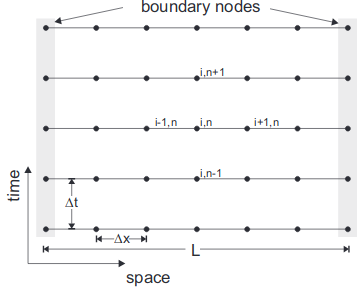
\includegraphics[width=0.5\linewidth]{1d-grid}
\caption{Finite difference discretization of the 1D heat problem}
\label{fig:1d-grid}
\end{figure}

The next step is to replace the continuous derivatives of equation \ref{eq:1DHeatEq} with their finite difference approximations. The derivative of $\phi$ versus time ($\frac{\partial \phi}{\partial t}$) can be approximated with a forward finite difference approximation as
\begin{equation}
\frac{\partial \phi}{\partial t} \approx \frac{\phi^{n+1}_{i}-\phi^{n}_{i}}{t^{n+1}-t^{n}} =\frac{\phi^{n+1}_{i}-\phi^{n}_{i}}{\Delta t}
\label{eq:timeDiscret}
\end{equation}
Here, $n$ represents the time step; and the subscript $i$ refers to the location. Both $n$ and $i$ are integers; $n$ varies from 1 to $n_t$ (total number of time steps) and $i$ varies from 1 to $n_x$ (total number of grid points in x-direction).The spatial derivative of equation \ref{eq:1DHeatEq} is replaced by a central finite difference approximation, i. e. 
\begin{equation}
\frac{\partial^2 \phi}{\partial x^2} = \frac{\partial}{\partial x}\frac{\partial \phi}{\partial x} \approx \frac{\frac{\phi^n_{i+1}-\phi^n_{i}}{\Delta x}-\frac{\phi^n_{i}-\phi^n_{i-1}}{\Delta x}}{\Delta x} = \frac{\phi^n_{i+1}-2\phi^n_{i}+\phi^n_{i-1}}{(\Delta x)^2}
\label{eq:spatialDiscret}
\end{equation}

Substituting equations \ref{eq:timeDiscret} and \ref{eq:spatialDiscret} into equation \ref{eq:1DHeatEq} gives:
\begin{equation}
\frac{\phi^{n+1}_{i}-\phi^{n}_{i}}{\Delta t}=D \frac{\phi^n_{i+1}-2\phi^n_{i}+\phi^n_{i-1}}{(\Delta x)^2}
\label{eq:1DheatDisc}
\end{equation}
Rearrenging the equation \ref{eq:1DheatDisc} gives an evolutionary equation for $\phi$, this method is called \textit{explicit scheme}.
\\
An alternative approach is an \textit{implicit finite difference scheme}, where the spatial derivatives $\frac{\partial^2 \phi}{\partial x^2}$ are evaluated at the new time step. The simplest implicit discretization of equation \ref{eq:1DHeatEq} is
\begin{equation}
\frac{\phi^{n+1}_{i}-\phi^{n}_{i}}{\Delta t}=D \frac{\phi^{n+1}_{i+1}-2\phi^{n+1}_{i}+\phi^{n+1}_{i-1}}{(\Delta x)^2}
\label{eq:1DheatDiscImplicit}
\end{equation}
A \textit{fully implicit} scheme where the time derivative is taken backward can be rearranged so that unknown terms are on the left and known terms are on the right
\begin{equation}
\label{eq:fullyImplicit}
-s \phi^{n+1}_{i+1} + (1+2s) \phi^{n+1}_{i} -s \phi^{n+1}_{i-1}=\phi^{n}_{i}
\end{equation}
where
\begin{equation}
\label{eq:s}
s=\frac{D \Delta t}{(\Delta x)^2}
\end{equation}
Note that in this case we no longer have an explicit relationship for $\phi^{n+1}_{i}$, $\phi^{n+1}_{i-1}$ and $\phi^{n+1}_{i+1}$. Instead, we have to solve a linear system of equations, which is discussed further below.
\\
We solve the heat equation (\ref{eq:1DHeatEq}) on the domain $0 \leq x \leq 1$ subject to the following boundary conditions for fixed temperature
%\begin{equation}

\begin{align}
\label{eq:BC1Dheat}
\phi(x=0)&=\phi_{left} \\
\phi(x=1)&=\phi_{right}
\end{align}
%\end{equation}
Starting with fixed temperature BCs (\ref{eq:BC1Dheat}), the boundary condition on the left boundary gives
\begin{equation}
\label{eq:BC1Dleft}
\phi_1=\phi_{left},
\end{equation}
and the one on the right 
\begin{equation}
\label{eq:BC1Dright}
\phi_{nx}=\phi_{right}.
\end{equation}
\\
Equation \ref{eq:fullyImplicit}, \ref{eq:BC1Dleft} and \ref{eq:BC1Dright} can be written in matrix form as
\begin{equation}
\label{eq:1DlinearSys}
A\vec{x}=\vec{b}.
\end{equation}
Acording to equation \ref{eq:fullyImplicit}, for a five-node grid, for example, the linear system becomes
%\begin{equation}
\begin{align*}
  grid \ point \ \# 1&: \qquad \phi^{n+1}_{1}= \qquad \phi^{n}_{1} &=\phi^{n}_{left} \\
  grid \ point \ \# 2&: -s \phi^{n+1}_{1} + (1+2s)\phi^{n+1}_{2} -s \phi^{n+1}_{3} &= \phi^{n}_{2} \\
  grid \ point \ \# 3&: -s \phi^{n+1}_{2} + (1+2s)\phi^{n+1}_{3} -s \phi^{n+1}_{4} &= \phi^{n}_{3} \\
  grid \ point \ \# 4&: -s \phi^{n+1}_{3} + (1+2s)\phi^{n+1}_{4} -s \phi^{n+1}_{5} &= \phi^{n}_{4} \\
  grid \ point \ \# 5&: \qquad \phi^{n+1}_{5}= \qquad \phi^{n}_{5} &=\phi^{n}_{right} \\
\label{eq:1D5node}
\end{align*}

%\end{equation}
thus the coefficient matrix A is
\begin{equation}
A = \begin{bmatrix}
       1 & 0 & 0 & 0 & 0 \\
	   -s & (1+2s) & -s & 0 & 0 \\
  	   0 & -s & (1+2s) & -s & 0  \\
  	   0 & 0 & -s & (1+2s) & -s  \\  	   
       0 & 0 & 0 & 0 & 1 \\
     \end{bmatrix}
\end{equation}
and vectors $\vec{x}$ and $\vec{b}$ are
\begin{equation}
x=\begin{bmatrix}
\phi^{n+1}_{1} \\ \phi^{n+1}_{2} \\ \phi^{n+1}_{3} \\ \phi^{n+1}_{4} \\ \phi^{n+1}_{5}
\end{bmatrix}
\quad
b=\begin{bmatrix}
\phi_{left} \\ \phi^{n}_{2} \\ \phi^{n}_{3} \\ \phi^{n}_{4} \\ \phi_{right}
\end{bmatrix}
\end{equation}
Note that matrix $A$ will have a unity entry on the diagonal and zero else for each node where Dirichlet (fixed temperature) boundary conditions apply.
\\
In case of the Dirichlet boundary condition, it is better if we get rid of the boundary points ($\phi_{left}$ and $\phi_{right}$) in the solution vector, that is we only take the evolving points. In this case, we have to take the effects of boundaries in a boundary condition vector on the right hand side of the equation \ref{eq:1DlinearSys}, and we can rewrite the equation as:
\begin{equation}
\label{eq:1DlinearSys+B.C.}
A'\vec{x'}=\vec{b'} + \vec{b.c.}
\end{equation} 
where, for a five-node grid the coefficient matrix is:
\begin{equation}
A' = \begin{bmatrix}
	   (1+2s) & -s & 0  \\
  	   -s & (1+2s) & -s \\
  	    0 & -s & (1+2s)   \\  	   
     \end{bmatrix}
\end{equation}
and vectors $\vec{x}$, $\vec{b}$, and $\vec{b.c.}$ are:
\begin{equation}
\vec{x'}=\begin{bmatrix}
 \phi^{n+1}_{2} \\ \phi^{n+1}_{3} \\ \phi^{n+1}_{4}
\end{bmatrix}
\quad
\vec{b'}=\begin{bmatrix}
\phi^{n}_{2} \\ \phi^{n}_{3} \\ \phi^{n}_{4}
\end{bmatrix}
\quad
\vec{b.c.}=s \begin{bmatrix}
\phi_{left} \\ 0 \\ \phi_{right}
\end{bmatrix}
\end{equation}
Linear system \ref{eq:1DlinearSys+B.C.} is like linear system \ref{eq:1DlinearSys}, but only for the evolving points (we have ignored the boundaries).
\\
Matrix $A$ also has an overall peculiar form because most entries off the diagonal are zero. This “sparseness” can be exploited by specialized linear algebra routines, both in terms of storage and speed. By avoiding computations involving zero entries of the matrix, much larger problems can be handled than would be possible if we were to store the full matrix. In particular, the fully implicit FD scheme leads to a “tridiagonal” system of linear equations that can be solved with various well known methods.
Thus solving a PDE is reduced to solve a system of linear equations. There are many methods of numerical solution of linear systems. 

\section{Numerical Solution of Linear Systems}
The problem of solving the equation $A \vec{x} = \vec{b} $ is to find the inverse of the coefficient matrix ($A^{-1}$). Multiplying $A^{-1}$ to the both sides of the equation leads to $A^{-1}A \vec{x}=A^{-1} \vec{b}$, with $A^{-1}A=\mathbf{1}$, it becomes $\vec{x} = A^{-1} \vec{b}$. So, it is clear that, all we have to do is to calculate the inverse of the coefficient matrix ($A^{-1}$).
\\
numerical methods for solving linear systems of equations can generally be divided into two classes \cite{allaire2008numerical} : 
\begin{itemize}
\item \textbf{Direct methods: } In the absence of rundoff error (assuming infinite precision!) such methods would yeild the exact solution, such as Gaussian Elimination, LU Decomposition, and etc.;
\item \textbf{Iterative methods: } These methods are consist of approximating solutions; start with a first approximation $x^{(0)}$ and compute iteratively a sequence of (hopefully increasingly better) approximations $x^{(i)}$, without ever reaching $x$. Gauss–Seidel Method, Conjugate Gradient Method, and etc. are some well known iterative methods.
\end{itemize}
We will explaine more about LU Decomposition, and Conjugate Gradient Method in the next sections.

\subsection{LU Decomposition}
The LU decomposition method consists in factorizing $A$ into a product of two triangular matrices $A=LU$, where $L$ is lower triangular and $U$ is upper triangular. This decomposition allows us to reduce the solution of the system $Ax = b$ to solving two triangular systems $Ly = b$ and $Ux = y$. Because $L$ and $U$ are triangular matrices finding the inverse matrix for them is much more easier than finding the inverse matrix for a general matrix, so the LU factorization provides a way of computing $A^{-1}$. Here is two-step procedure to find the inverse of a matrix $A$:
\begin{enumerate}
\item Find the LU decomposition $A = LU$;
\item Find the inverse of $A^{-1} = U^{-1}L^{-1}$ by inverting the matrices $U$ and $L$.
\end{enumerate}
There are two subroutines in the Linear Algebra PACKage (LAPACK) which do the same job:
\begin{itemize}
\item the \textbf{SGETRF} subroutine \footnote{check \texttt{www.netlib.org} for more information on these subroutines} computes an LU factorization of a general M-by-N matrix A using partial pivoting with row interchanges.
\item the \textbf{SGETRI} subroutine computes the inverse of a matrix using the LU factorization computed by SGETRF.
\end{itemize}

Our algorithm for solving the one-dimensional heat equation using LU fectorization is summarised as:
\begin{enumerate} % [noitemsep] removes whitespace between the items for a compact look
\item assembling system in a desired boundary conditions and building the coeficient matrix($A$);
\item calculating the inverse of the coeficient matrix($A^{-1}$) using LU decomposition;
\item setting the initial conditions;
\item loop over time:
	\begin{enumerate}
		\item $\phi^{n} = A^{-1} \phi^{n-1}$;
	\end{enumerate}
\end{enumerate}

\subsection{Conjugate Gradient Algorithm}
The classic Conjugate Gradient non-stationary iterative algorithm as defined in \cite{dongarra1991solving} and references therein can be applied to solve symmetric positive-definite matrix equations. They are preferred over simple Gaussian algorithms because of their faster convergence rate if $A$ is very large and sparse.
\\
consider the prototype problem $A \vec{x} = \vec{b}$ to be solved for $\vec{x}$ which can be expressed in the form of iterative equations for the solution $\vec{x}$ and residual (gradient) $\vec{r}$ \cite{hawick1995conjugate}. 

\begin{equation}
\vec{x}^{k} = \vec{x}^{k-1} +\alpha^{k} \vec{p}^{k}
\label{eq:CGx}
\end{equation}
\begin{equation}
\vec{r}^{k} = \vec{r}^{k-1} -\alpha^{k} \vec{q}^{k}
\label{eq:CGr}
\end{equation}

where  the new value $vec{x}$ is a function of its old value, the scaler step size $\alpha$ and the search direction vector $\vec{p}$ at the $k$'th iteration and $\vec{q^k}=A\vec{p^k}$.
\\
The values of $x$ are guaranteed to converge in, at most, $n$ iterations, where $n$ is the order of the system, unless the problem is ill-conditioned in which case roundoff errors often prevent the algorithm from furnishing a suffciently precise solution at the $n$th step. In well-conditioned problems, the number of iterations necessary for satisfactory convergence of the conjugate gradient method can be much less than the order of the system. Therefore, the iterative procedure is continued until the residual $\vec{r}^k=\vec{b}^k-A\vec{x}^k$ meets some stopping criterion, typically of the form: $\| \vec{r}^k \| \leq \text{tol.}$ ($\text{tol.} is$ a tolerance level). The CG algorithm uses:
\begin{equation}
\alpha = (\vec{r}^k . \vec{r}^k ) / (\vec{p}^k . A \vec{p}^k)
\label{eq:CGalpha}
\end{equation}
with the search directions chosen using:
\begin{equation}
\vec{p}^k=\vec{r}^{k-1}+ \beta^{k-1} \vec{p}^{k-1}
\label{eq:CGsearchDir}
\end{equation}
with 
\begin{equation}
\beta^{k-1}= ( \vec{r}^{k-1} . \vec{r}^{k-1} ) / ( \vec{p}^{k-2} . A \vec{p}^{k-2} )
\label{eq:CGbeta}
\end{equation}
which ensures that the search directions form an A-orthogonal system.
The non-preconditioned CG algorithm for the initial "guessed" solution vector $\vec{x}^0 = 0$ is summarised as:
\\
$\vec{p} =\vec{r}=\vec{b}; \ \vec{x}=0 ; \ \vec{q}=A \vec{p}$ \\
$\rho = \vec{r} . \vec{r} ; \ \alpha = \rho /( \vec{p} . \vec{q} )$\\
$\vec{x} = \vec{x} + \alpha \vec{p} ; \ \vec{r}= \vec{r} - \alpha \vec{q}$\\
$ \textbf{DO} \ k=2,Niter$\\
$ \rightarrow \rho_0 = \rho ; \ \rho= \vec{r} . \vec{r} ; \ \beta = \rho_0 / \rho $\\
$ \rightarrow  \vec{p}=\vec{r} + \beta \vec{p} ; \ \vec{q}= A \vec{p}$ \\
$ \rightarrow  \alpha = \rho / ( \vec{p} . \vec{q})$\\
$ \rightarrow  \vec{x}=\vec{x}+\alpha \vec{p}; \ \vec{r}=\vec{r}-\alpha\vec{q}$\\
$ \rightarrow  \textbf{IF} \  \text{(stop criterion)} \ \textbf{EXIT} $\\
$ \textbf{END DO}$\\

The Conjugate Gradient method involves one matrix-vector product, three vector updates, and two inner products per iteration. Implementation of this algorithm requires storage for four vectors: $\vec{x}$ , $\vec{r}$ , $\vec{r}$ and $\vec{q}$ as well as the matrix $A$ and working scalars $\alpha$ and $\beta$. 
\\
Note that there are other CG Algorithms too, such as Bi-Conjugate Gradient (BiCG) method which can be applied to non-symmetric matrices.
\\
Our algorithm for solving the one-dimensional heat equation using CG is summarised as:
\begin{enumerate} % [noitemsep] removes whitespace between the items for a compact look
\item Assembling system in a desired boundary conditions and building the coeficient matrix($A$);
\item setting the initial conditions;
\item loop over time:
	\begin{enumerate}
		\item Using CG to fing the $\phi$ for the next timestep;
	\end{enumerate}
\end{enumerate}
Also there are maximum tolrrance and maximum iteration for the CG algorithm to be sure whenever each one satisfied the CG loop will break.


\begin{figure}[ht]
  \centering
  \begin{minipage}{.7\linewidth}
    \begin{algorithm}[H]
      \SetAlgoLined
      \KwData{this text}
      \KwResult{how to write algorithm with \LaTeX2e }
      initialization\;
      \While{not at end of this document}{
        read current\;
        \eIf{understand}{
          go to next section\;
          current section becomes this one\;
        }{
          go back to the beginning of current section\;
        }
      }
      \caption{How to write algorithms}
    \end{algorithm}
  \end{minipage}
\end{figure}

%\input{sections/03-L}
\section{Results for one-dimensional heat equation}
We have tried both LU decomposition and CG methods for solving one-dimentional heat equation, to compare their efficiency.

The parameters set to $D=1.0$, $dt= 2.0^{-8.0}$, $x=[0,1.1]$, $n_x=10$, and for initial condition we have $phi(x-0.5)=100.0$ (figure \ref{fig:1d-initial_condition}). Solving $\phi$ for the next timesteps leads to figures \ref{fig:1d-1dt} and \ref{fig:1d-tdt}.

\begin{figure}
     \centering
     \begin{subfigure}[b]{0.45\textwidth}
         \centering
         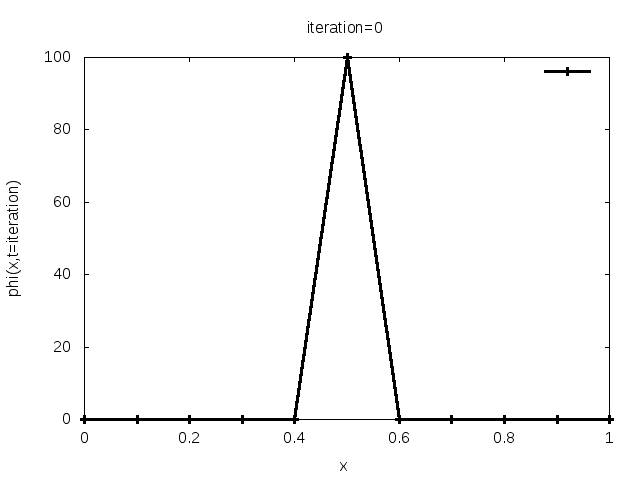
\includegraphics[width=\textwidth]{1Dfig/0}
		\caption{initial condition for one-dimensional heat equation}
         \label{fig:1d-initial_condition}
     \end{subfigure}
 %    \hfill
     \begin{subfigure}[b]{0.45\textwidth}
         \centering
         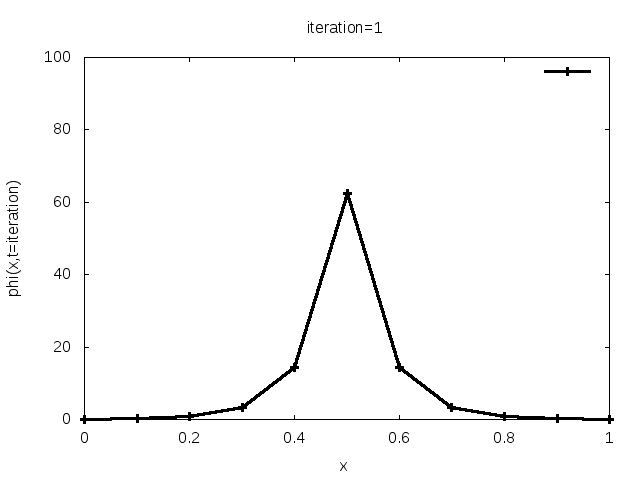
\includegraphics[width=\textwidth]{1Dfig/1}
		\caption{the heat distribution after one timestep.}
         \label{fig:1d-1dt}
     \end{subfigure}
%     \hfill
     \begin{subfigure}[b]{0.5\textwidth}
         \centering
         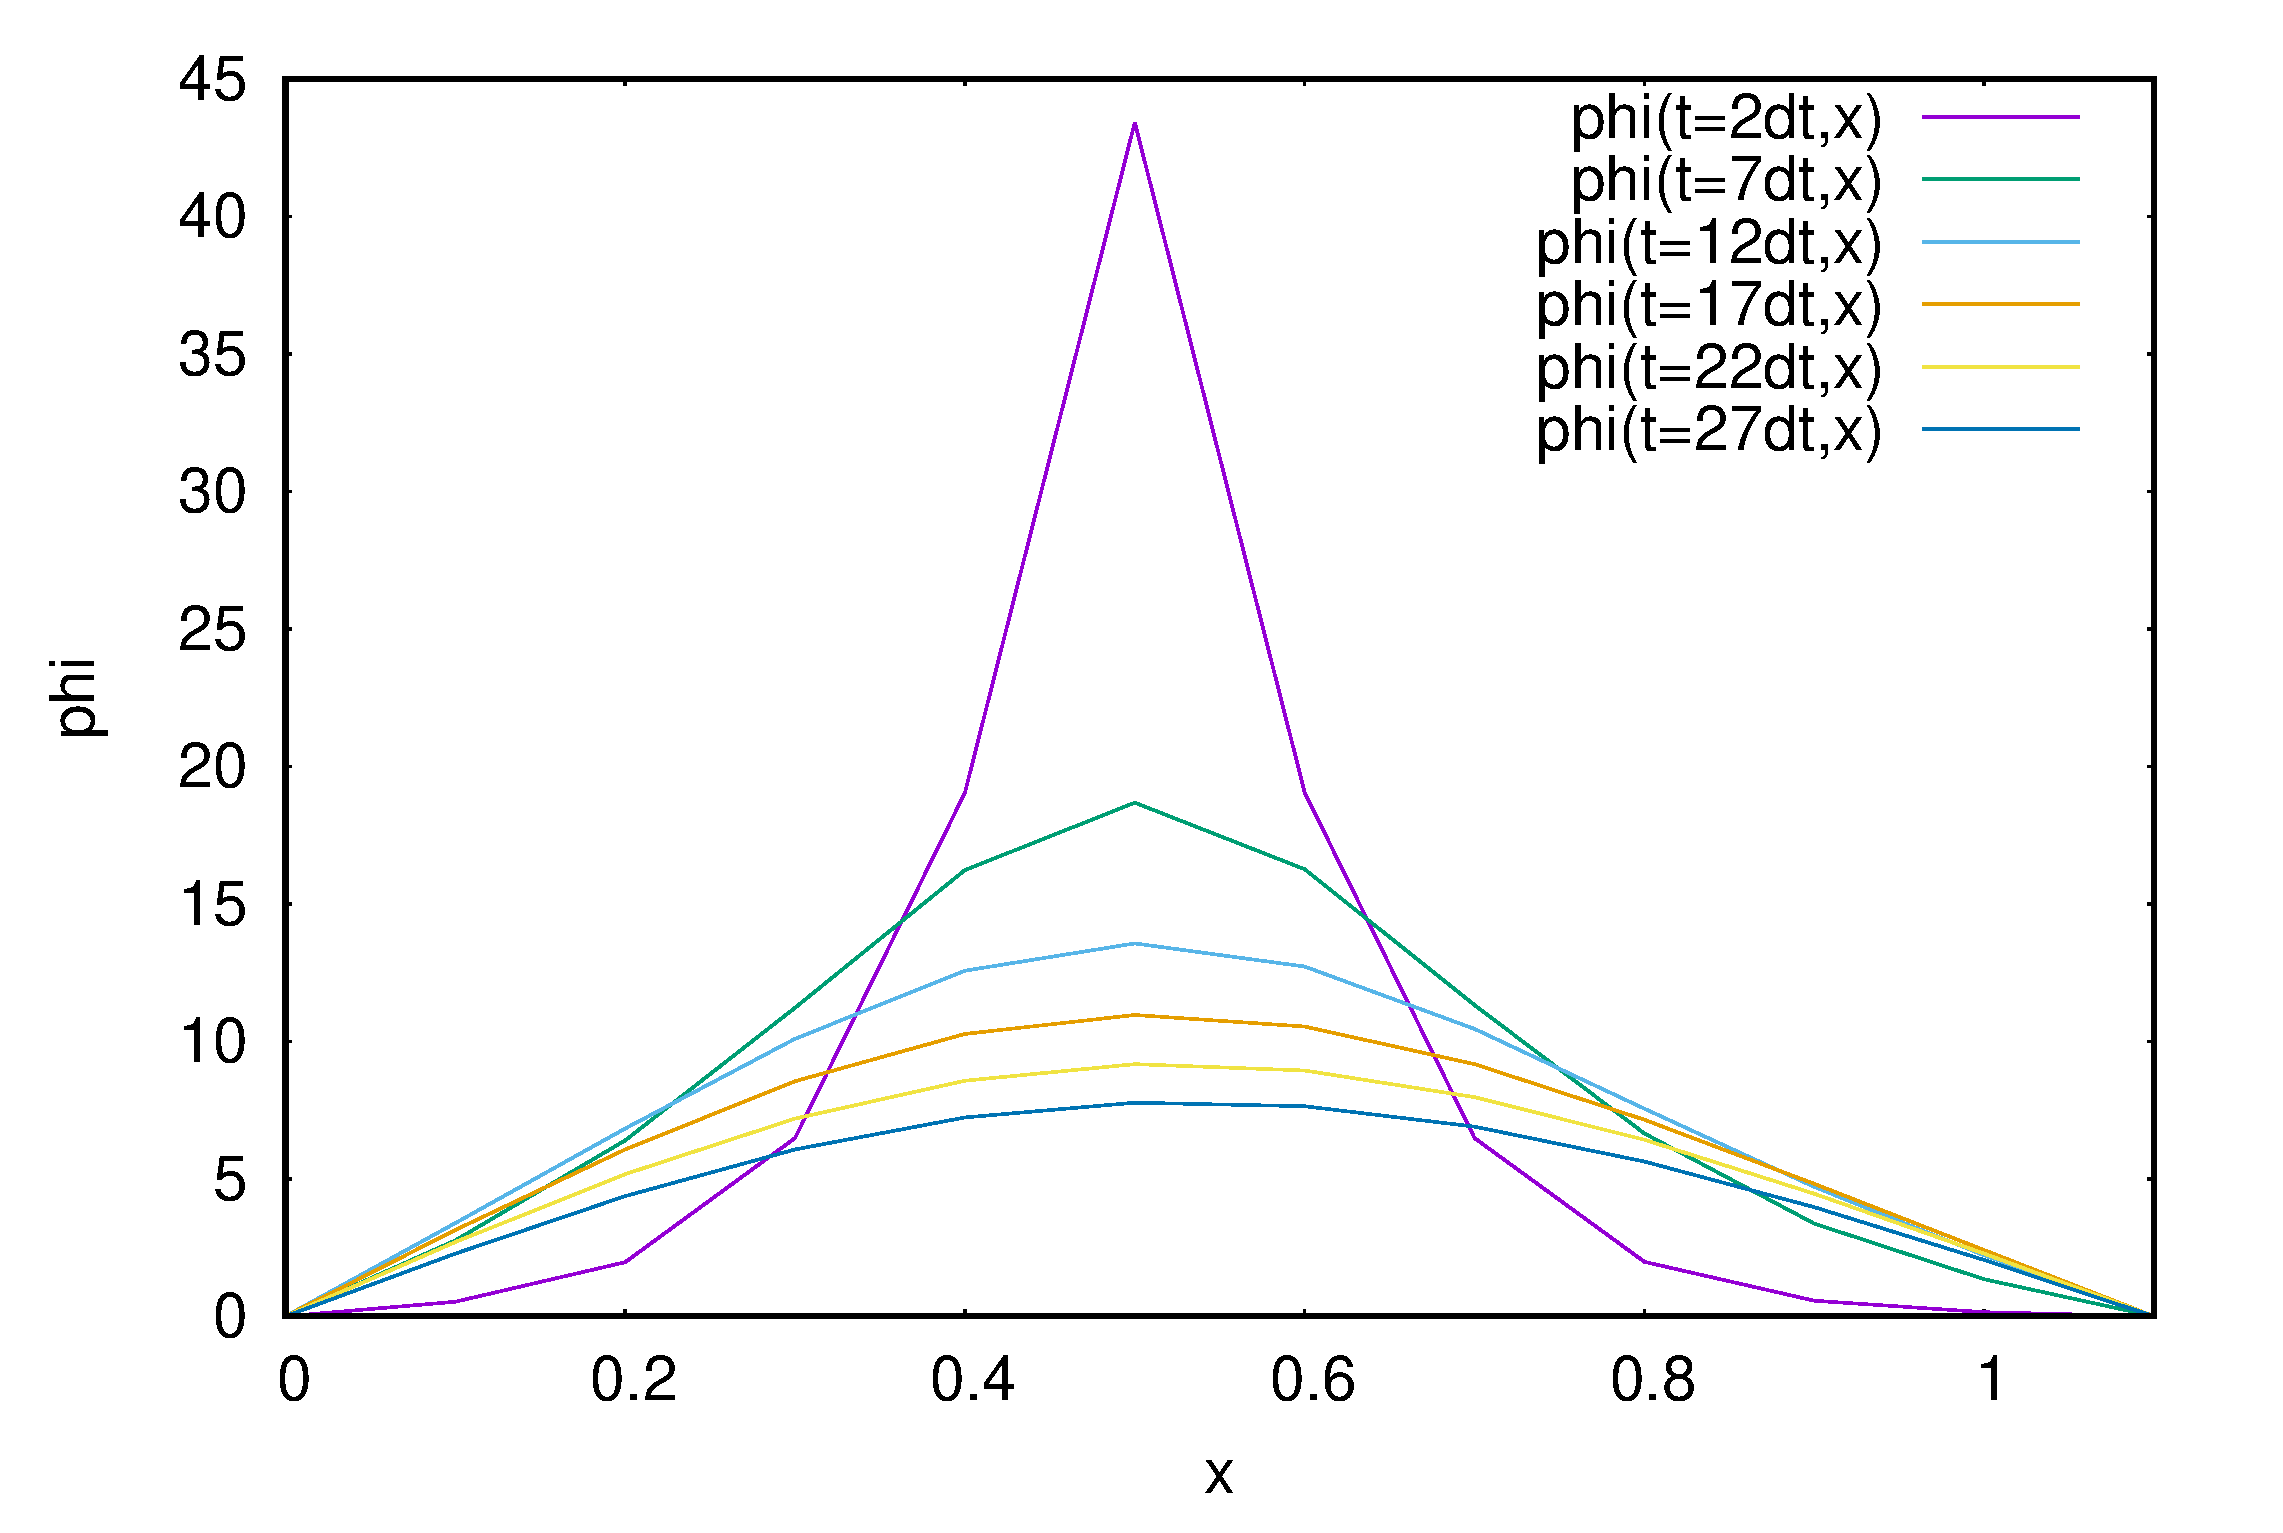
\includegraphics[width=\textwidth]{1Dfig/result1D}
		 \caption{the heat distribution after several timesteps.}
		\label{fig:1d-tdt}
     \end{subfigure}
     
        \caption{solving one-dimensional heat equation using LU factorization.}
        \label{fig:1d-du}
\end{figure}


%\begin{figure}[h]\centering
%%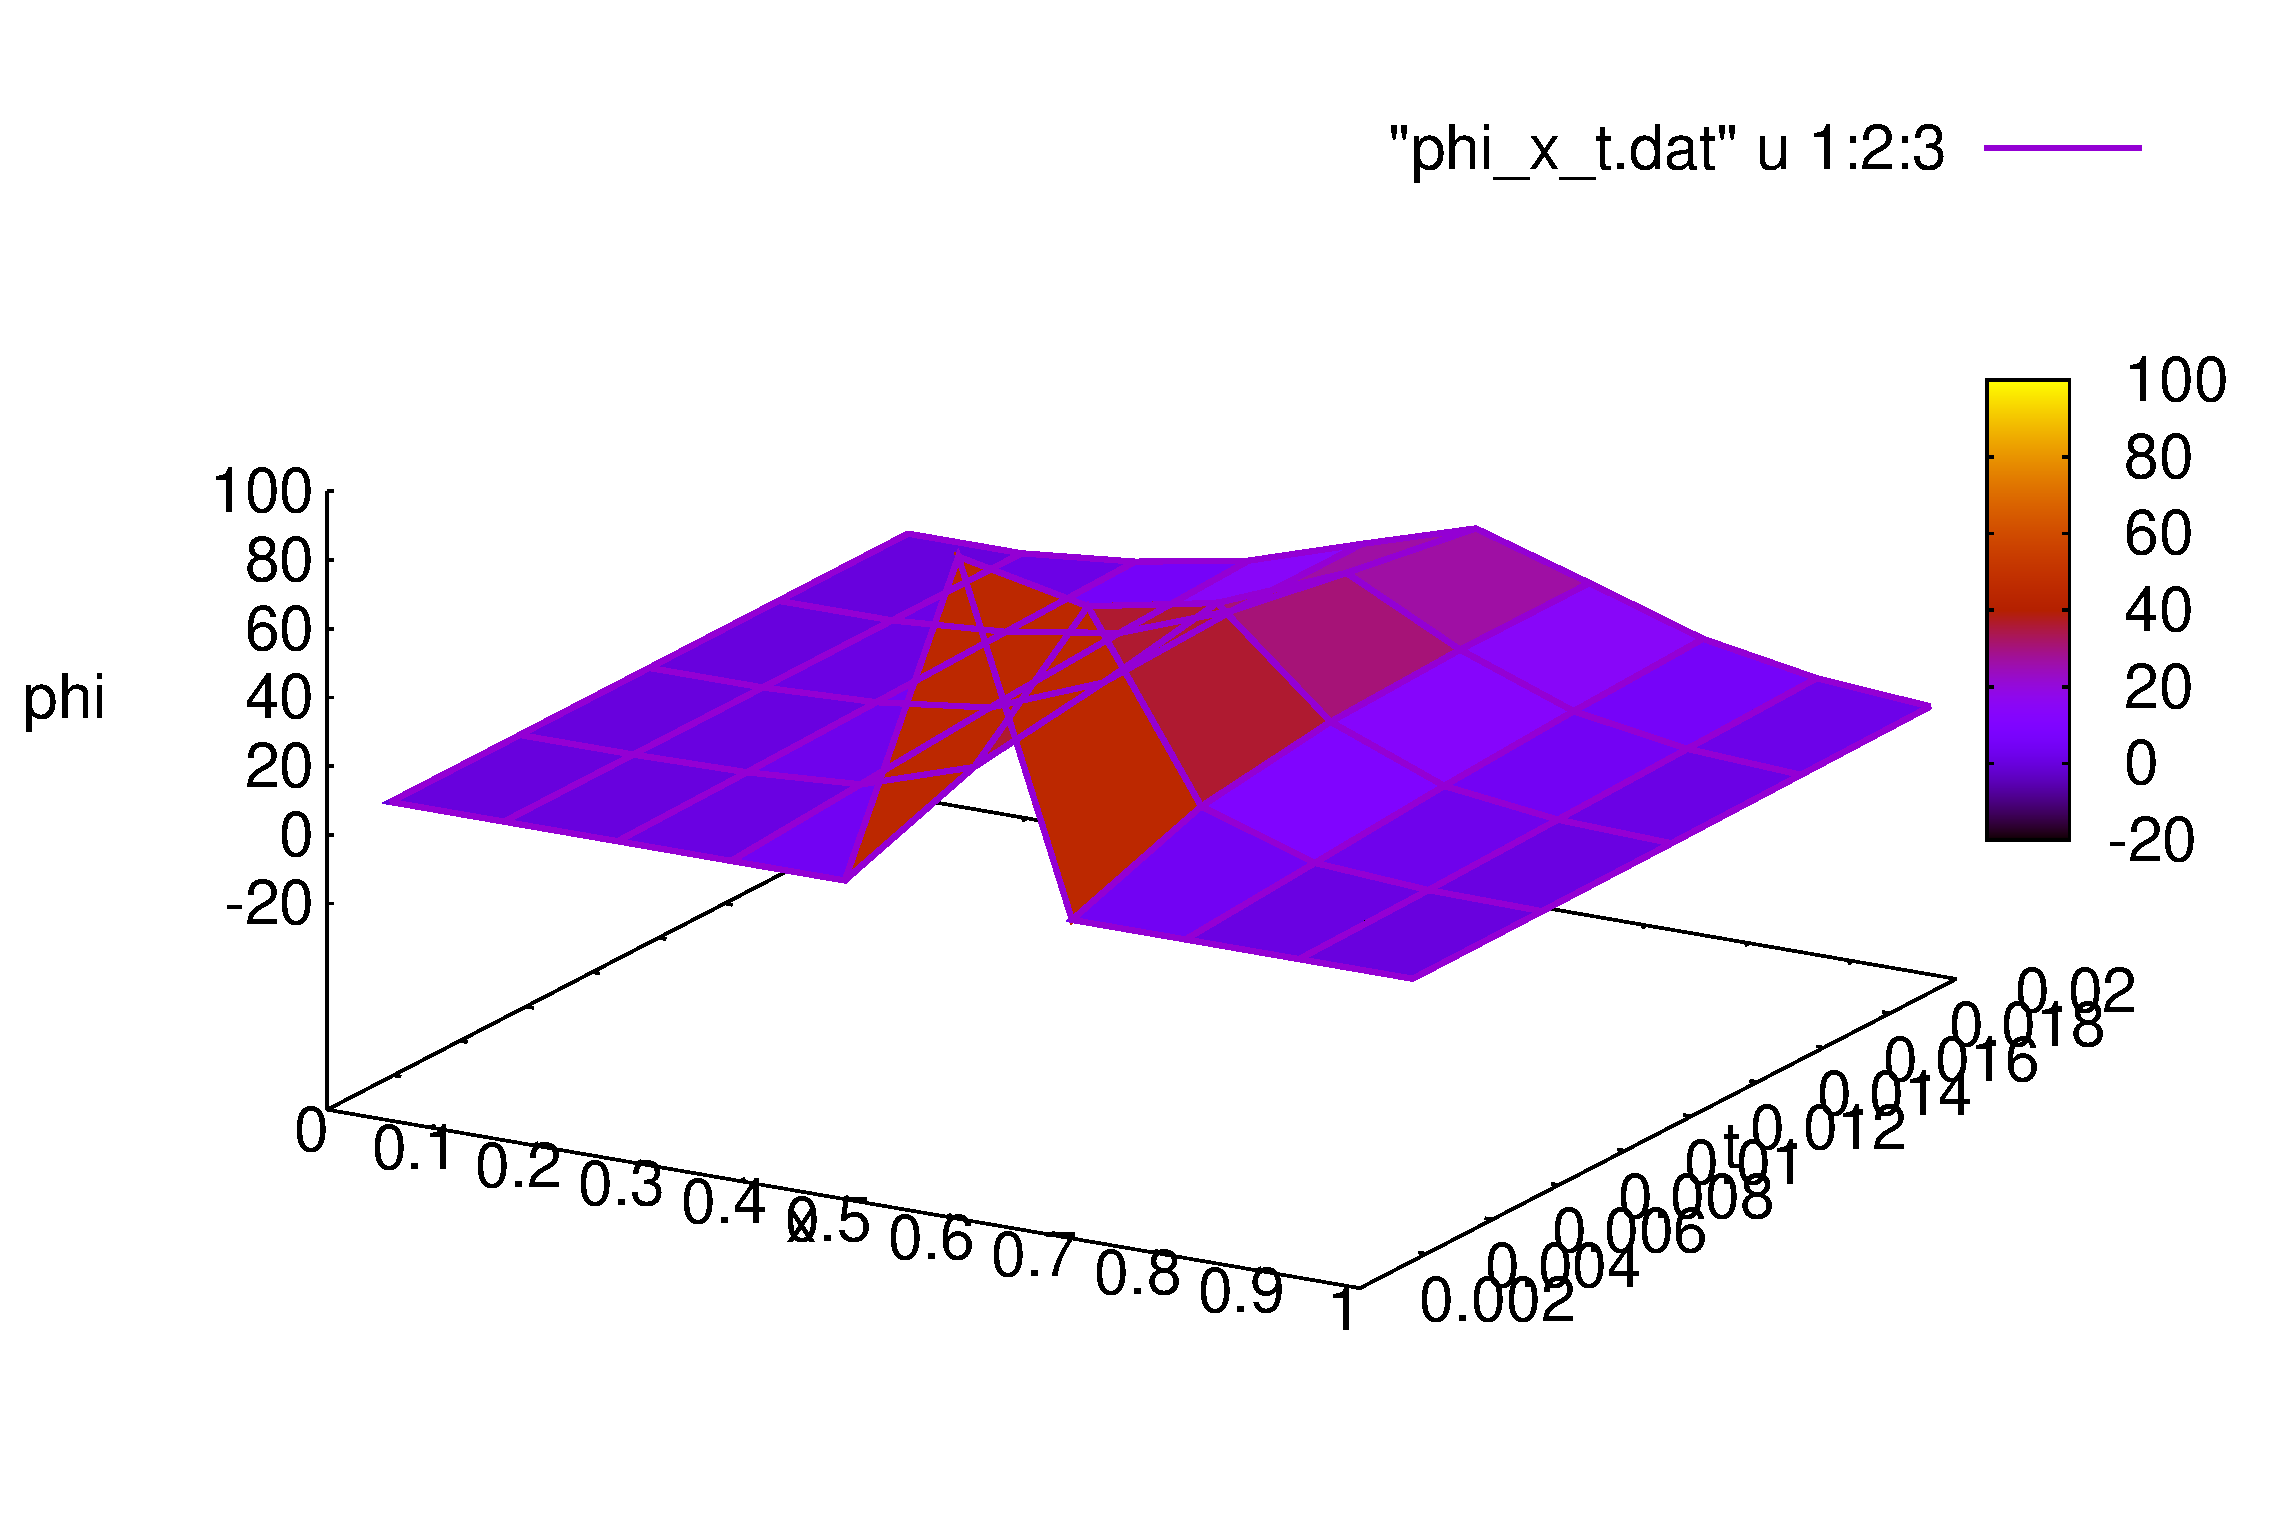
\includegraphics[width=\linewidth]{1Dfig/result1D_CG}
%\caption{solution $\phi(t,x)$ for one-dimensional heat equation at several timesteps using CG algorithm.}
%\label{fig:1d-t-CG}
%\end{figure}

\begin{figure}
     \centering
     \begin{subfigure}[b]{0.45\textwidth}
         \centering
         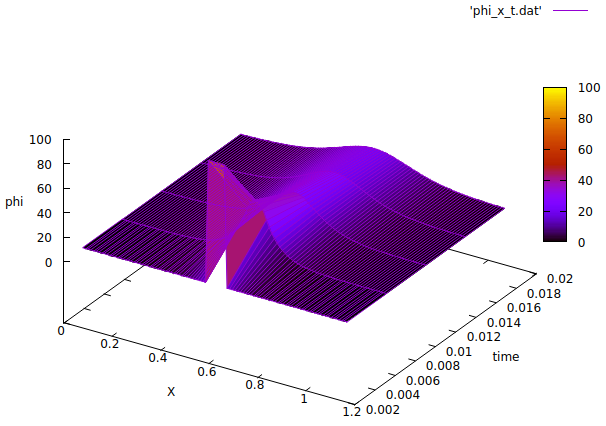
\includegraphics[width=\textwidth]{1Dfig/result1D_CG-2}
		\caption{the heat distribution over time}
		\label{fig:1d-t-CG-2}
     \end{subfigure}
     \hfill
     \begin{subfigure}[b]{0.45\textwidth}
         \centering
         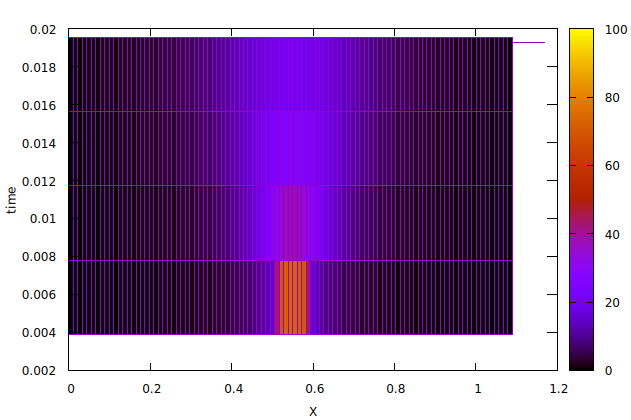
\includegraphics[width=\textwidth]{1Dfig/result1D_CG-2-map}
		\caption{the heat distribution map over time.}
	\label{fig:1d-t-CG-2-map}
     \end{subfigure}
     
        \caption{solving one-dimensional heat equation using CG method.}
        \label{fig:1d-CG}
\end{figure}




We can study several initial conditions to get a deeper insight into the different diffusion problems(figures \ref{fig:1d-t-CG-LR} and \ref{fig:1d-t-CG-gaussianPulse}).

\begin{figure}
     \centering
     \begin{subfigure}[b]{0.45\textwidth}
         \centering
         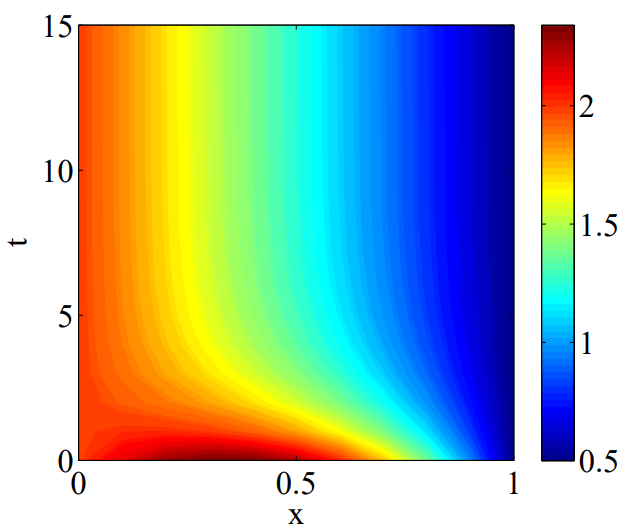
\includegraphics[width=\textwidth]{1Dfig/result1D_CG_LR}
		 \caption{Contour plot of the heat distribution, $\phi(0,t)=T_l$, $\phi(L,t)=T_r$.}
 		 \label{fig:1d-t-CG-LR}
     \end{subfigure}
     \hfill
     \begin{subfigure}[b]{0.45\textwidth}
         \centering
         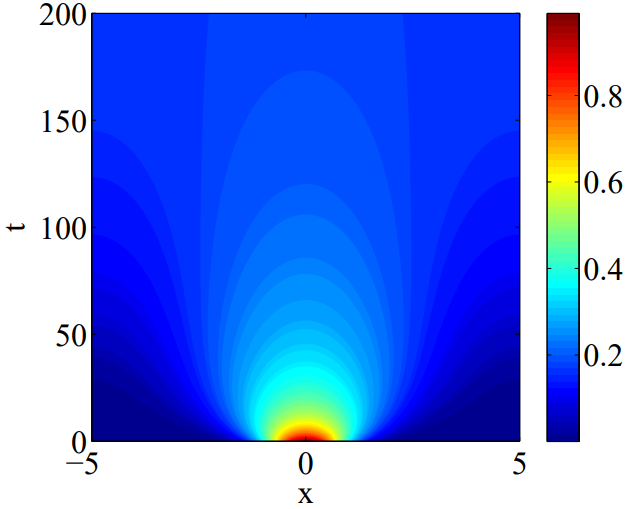
\includegraphics[width=\textwidth]{1Dfig/result1D_CG_gaussianPulse}
\caption{Contour plot of the diffusion of the initial Gauss pulse.}
\label{fig:1d-t-CG-gaussianPulse}
     \end{subfigure}
     
        \caption{solving one-dimensional heat equation using CG method.}
        \label{fig:1d-CG}
\end{figure}

%todo
\textbf{todo:} compare the run time of two methods.
\\

In the next section we will explaine all the issues and considerations for the two-dimentional heat equation.\\
\section{Two-dimensional diffusion equation}
Now we consider two-dimentional diffusion equation; if the diffusion coefficient ($D$) is costant, then  the two-dimensional diffusion equation reduces to the following linear equation:
\begin{equation}
\label{eq:2Dheat}
\frac{\partial \phi(\vec{r},t)}{\partial t}= D \nabla^2 \phi(\vec{r},t)
\end{equation}
and if we assume that $\vec{r}=(x,z)$ it becomes to
\begin{equation}
\label{eq:2DheatOtherForm}
\frac{\partial \phi(x,z,t)}{\partial t}= D \left( \frac{\partial ^2 \phi(x,z,t)}{\partial x^2} +\frac{\partial ^2 \phi(x,z,t)}{\partial z^2} \right).
\end{equation}

\begin{figure}[ht]\centering
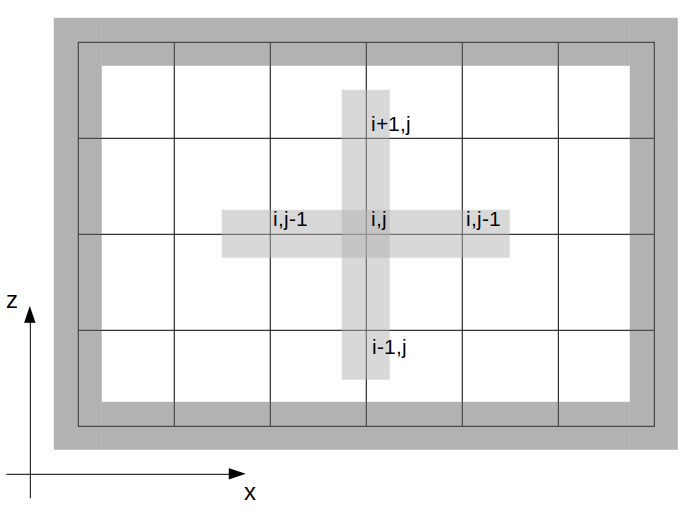
\includegraphics[width=\linewidth]{2d-grid}
\caption{Finite difference discretization of the 2D heat problem}
\label{fig:2d-grid}
\end{figure}

According to the previous explanation on Taylor-series expansion and Linearization of PDEs, if we employ a fully implicit, unconditionally stable discretization scheme as we have done for the 1D equation , equation \ref{eq:2DheatOtherForm} can be written as

%\begin{equation}
\begin{align*}
\frac{\phi^{n+1}_{i,j}-\phi^{n}_{i,j}}{\Delta t} = D & ( \frac{\phi^{n+1}_{i,j+1}-2\phi^{n+1}_{i,j}+\phi^{n+1}_{i,j-1}}{(\Delta x)^2} \\ &+ \frac{\phi^{n+1}_{i+1,j}-2\phi^{n+1}_{i,j}+\phi^{n+1}_{i-1,j}}{(\Delta z)^2} )
\end{align*}
%\end{equation}
Rearranging terms with $n + 1$ on one side and terms with $n$ on the other side gives
%\begin{equation}
\begin{align*}
&\phi^{n}_{i,j} = \\
&-s_z \phi^{n+1}_{i+1,j}-s_x \phi^{n+1}_{i,j+1} +(1+2s_z+2s_x) \phi^{n+1}_{i,j} -s_z \phi^{n+1}_{i-1,j}-s_x \phi^{n+1}_{i,j-1}
\label{eq:2Ddescrete}
\end{align*}
%\end{equation}
As in the 1D case, we have to write these equations in a matrix $A$ and a vector $\vec{b}$. From a practical point of view, this is a bit more complicated than in the 1D case, since we have to deal with “book-keeping” issues, i.e. the mapping of $\phi_{i,j}$ to the entries of a vector $\Phi_k$. 
\\
If a 2D scalar field is to be solved for with an equivalent vector $\Phi$, the nodes have to be numbered continuously, for example as in Figure \ref{fig:2d-grid-mapping}. The derivative versus x-direction is then e.g.

\begin{figure}[ht]\centering
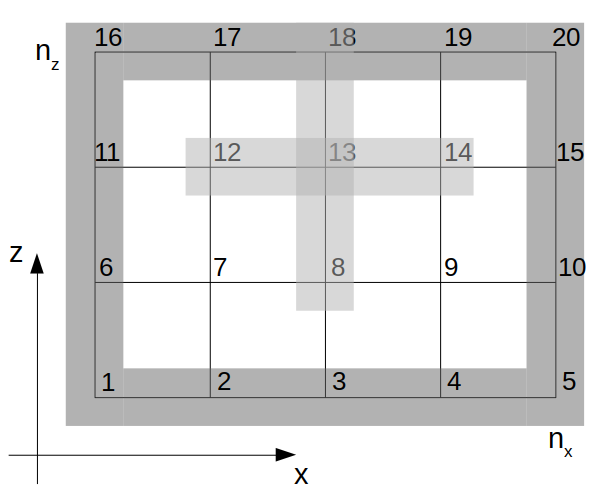
\includegraphics[width=\linewidth]{2d-grid-mapping}
\caption{Numbering scheme for a 2D grid with $n_x = 5$ and $n_z = 4$.}
\label{fig:2d-grid-mapping}
\end{figure}

\begin{equation}
\frac{\partial^2 \phi}{\partial x^2}|_{i=3,j=3}= \frac{1}{(\Delta x)^2}(\Phi_{14}-2\Phi_{13}+\Phi_{12})
\label{eq:grid19x}
\end{equation}
and the derivative versus z-direction is given by
\begin{equation}
\frac{\partial^2 \phi}{\partial z^2}|_{i=3,j=3}= \frac{1}{(\Delta z)^2}(\Phi_{18}-2\Phi_{13}+\Phi_{8})
\label{eq:grid19z}
\end{equation}

If $n_x$ are the number of grid points in x-direction and $n_z$ the number of points in z-direction, we can write equations \ref{eq:grid19x} and \ref{eq:grid19z} in a more general way as:
\begin{equation}
\frac{\partial^2 \phi}{\partial x^2}|_{i,j}= \frac{1}{(\Delta x)^2}(\phi_{(i-1)n_x+j+1}-2\phi_{(i-1)n_x+j}+\phi_{(i-1)n_x+j-1})
\label{eq:gridKx}
\end{equation}
\begin{equation}
\frac{\partial^2 \phi}{\partial z^2}|_{i,j}= \frac{1}{(\Delta z)^2}(\phi_{in_x+j}-2\phi_{(i-1)n_x+j}+\phi_{(i-2)n_x+j})
\label{eq:gridKz}
\end{equation}

As an example, for a $4 \times 5$ grid there are $20$ grid points but $14$ of them are boundary points (located at left, right, top, and bottom) which do not have evolution. There are only $6$ middle points that have evolution in time. Thus, the coefficint matrix $A$ is $20 \times 20$, and on $14$ rows we have just one non-zero element (corresponding to the boundary condition).
\\
According to equation \ref{eq:2Ddescrete}, for a $4 \times 5$ grid, for example, at the boundary points the linear system becomes
%\begin{equation}
\begin{align}
bottom &: \qquad \phi^{n+1}_{1,1}= \phi^{n+1}_{1,2}=\phi^{n+1}_{1,3}=\phi^{n+1}_{1,4}=\phi^{n+1}_{1,5}=\phi_{bottom} \\
top &: \qquad \phi^{n+1}_{4,1}=\phi^{n+1}_{4,2}=\phi^{n+1}_{4,3}=\phi^{n+1}_{4,4}=\phi^{n+1}_{4,5} = \phi_{top} \\
left &: \qquad \phi^{n+1}_{2,1}=\phi^{n+1}_{3,1}=\phi_{left} \\
right &: \qquad \phi^{n+1}_{2,5}=\phi^{n+1}_{3,5}= \phi_{right} \\
\label{eq:2D45boundary}
\end{align}
%\end{equation}
\begin{align}
grid \ point \ 2,2 &:-s_z \phi^{n+1}_{3,2} -s_x \phi^{n+1}_{2,3} +(1+s_z+s_x) \phi^{n+1}_{2,2} -s_z \phi^{n+1}_{1,2} -s_x \phi^{n+1}_{2,1}  = \phi^{n+1}_{2,2} \\
grid \ point \ 2,3 &:-s_z \phi^{n+1}_{3,3} -s_x \phi^{n+1}_{2,4} +(1+s_z+s_x) \phi^{n+1}_{2,3} -s_z \phi^{n+1}_{1,3} -s_x \phi^{n+1}_{2,2}  = \phi^{n+1}_{2,3} \\
grid \ point \  2,4 &:-s_z \phi^{n+1}_{3,5} -s_x \phi^{n+1}_{2,5} +(1+s_z+s_x) \phi^{n+1}_{2,4} -s_z \phi^{n+1}_{1,4} -s_x \phi^{n+1}_{2,3}  = \phi^{n+1}_{2,4} \\
grid \ point \ 3,2 &:-s_z \phi^{n+1}_{4,2} -s_x \phi^{n+1}_{3,3} +(1+s_z+s_x) \phi^{n+1}_{3,2} -s_z \phi^{n+1}_{2,2} -s_x \phi^{n+1}_{3,1}  = \phi^{n+1}_{3,2} \\
grid \ point \ 3,3 &:-s_z \phi^{n+1}_{4,3} -s_x \phi^{n+1}_{3,4} +(1+s_z+s_x) \phi^{n+1}_{3,3} -s_z \phi^{n+1}_{2,3} -s_x \phi^{n+1}_{3,2}  = \phi^{n+1}_{3,3} \\
grid \ point \ 3,4 &:-s_z \phi^{n+1}_{4,4} -s_x \phi^{n+1}_{3,5} +(1+s_z+s_x) \phi^{n+1}_{3,4} -s_z \phi^{n+1}_{2,4} -s_x \phi^{n+1}_{3,3}  = \phi^{n+1}_{3,4} \\
\label{eq:2D45middle}
\end{align}
%\end{equation}
%\end{table*}


and the linear system for the $6$ other points located between the boundaries becomes \ref{eq:2D45middle}.  
\\

%\begin{table*}[ht]
%\begin{equation}

As we explained previously the “book-keeping” issues, i.e. the mapping of $\phi_{i,j}$ to the vector $\Phi_k$ , vectors $\vec{x}$ and $\vec{b}$ become equation \ref{eq:2D45xb}.

\begin{equation}
x= \begin{bmatrix}
	\phi^{n+1}_{1,1} \\ \phi^{n+1}_{1,2} \\ \phi^{n+1}_{1,3} \\ \phi^{n+1}_{1,4} \\ \phi^{n+1}_{1,5} \\ \phi^{n+1}_{2,1} \\ \phi^{n+1}_{2,2} \\ \phi^{n+1}_{2,3} \\ \phi^{n+1}_{2,4} \\ \phi^{n+1}_{2,5} \\ \phi^{n+1}_{3,1} \\ \phi^{n+1}_{3,2} \\ \phi^{n+1}_{3,3} \\ \phi^{n+1}_{3,4} \\ \phi^{n+1}_{3,5} \\ \phi^{n+1}_{4,1} \\ \phi^{n+1}_{4,2} \\ \phi^{n+1}_{4,3} \\ \phi^{n+1}_{4,4} \\ \phi^{n+1}_{4,5} 
\end{bmatrix}
=
   \begin{bmatrix}
	\Phi^{n+1}_{1} \\ \Phi^{n+1}_{2} \\ \Phi^{n+1}_{3} \\ \Phi^{n+1}_{4} \\ \Phi^{n+1}_{5} \\ \Phi^{n+1}_{6} \\ \Phi^{n+1}_{7} \\ \Phi^{n+1}_{8} \\ \Phi^{n+1}_{9} \\ \Phi^{n+1}_{10} \\ \Phi^{n+1}_{11} \\ \Phi^{n+1}_{12} \\ \Phi^{n+1}_{13} \\ \Phi^{n+1}_{14} \\ \Phi^{n+1}_{15} \\ \Phi^{n+1}_{16} \\ \Phi^{n+1}_{17} \\ \Phi^{n+1}_{18} \\ \Phi^{n+1}_{19} \\ \Phi^{n+1}_{20} 
   \end{bmatrix}
    , \qquad \quad
b= \begin{bmatrix}
	\phi^{n}_{1,1} \\ \phi^{n}_{1,2} \\ \phi^{n}_{1,3} \\ \phi^{n}_{1,4} \\ \phi^{n}_{1,5} \\ \phi^{n}_{2,1} \\ \phi^{n}_{2,2} \\ \phi^{n}_{2,3} \\ \phi^{n}_{2,4} \\ \phi^{n}_{2,5} \\ \phi^{n}_{3,1} \\ \phi^{n}_{3,2} \\ \phi^{n}_{3,3} \\ \phi^{n}_{3,4} \\ \phi^{n}_{3,5} \\ \phi^{n}_{4,1} \\ \phi^{n}_{4,2} \\ \phi^{n}_{4,3} \\ \phi^{n}_{4,4} \\ \phi^{n}_{4,5} 
\end{bmatrix}
=
\begin{bmatrix}
	\phi_{bottom} \\ \phi_{bottom} \\ \phi_{bottom} \\ \phi_{bottom} \\ \phi_{bottom} \\ \phi_{left} \\ \Phi^{n}_{7} \\ \Phi^{n}_{8} \\ \Phi^{n}_{9} \\ \phi_{right} \\ \phi_{left} \\ \Phi^{n}_{12} \\ \Phi^{n}_{13} \\ \Phi^{n}_{14} \\ \phi_{right} \\ \phi_{top} \\ \phi_{top} \\ \phi_{top} \\ \phi_{top} \\ \phi_{top} 
\end{bmatrix}
\label{eq:2D45xb}
\end{equation}
And the coefficient matrix, $A$, is \ref{eq:2D45A}. 
\\ 
Now two-dimentional heat equation (\ref{eq:2Dheat}) on a $5 \times 4$ grid reduced to a linear system $A\vec{x}=\vec{b}$, with  $\vec{x}$, $\vec{b}$, and $A$ are given by equations \ref{eq:2D45xb}, \ref{eq:2D45A}. 
\\
This is the way to find the coefficient matrix, and notice that for different boundary conditions we should modify some elements in the coefficient matrix. You can easily understand the pattern in the coefficient matrix, it will help you to build it in your code.
\\
Now that we know how to build the coefficient matrix for two-dimentional problem, it is the time to check what we have orgnized so far. 

\pagebreak

\begin{landscape}% Landscape page
\begin{flushleft}
 	The coefficient matrix, $A$, for a $5 \times 4$ grid is
\end{flushleft}

        \centering % Center table
\begin{equation}
\setcounter{MaxMatrixCols}{20}
\footnotesize{
A = \begin{bmatrix}
    \begin{array}{ccccc|ccccc|ccccc|ccccc}
       1 & 0 & 0 & 0 & 0 & 0 & 0 & 0 & 0 & 0 & 0 & 0 & 0 & 0 & 0 & 0 & 0 & 0 & 0 & 0 \\ %1
       0 & 1 & 0 & 0 & 0 & 0 & 0 & 0 & 0 & 0 & 0 & 0 & 0 & 0 & 0 & 0 & 0 & 0 & 0 & 0 \\ %2
       0 & 0 & 1 & 0 & 0 & 0 & 0 & 0 & 0 & 0 & 0 & 0 & 0 & 0 & 0 & 0 & 0 & 0 & 0 & 0 \\ %3
       0 & 0 & 0 & 1 & 0 & 0 & 0 & 0 & 0 & 0 & 0 & 0 & 0 & 0 & 0 & 0 & 0 & 0 & 0 & 0 \\ %4
       0 & 0 & 0 & 0 & 1 & 0 & 0 & 0 & 0 & 0 & 0 & 0 & 0 & 0 & 0 & 0 & 0 & 0 & 0 & 0 \\ %5
         \hline
       0 & 0 & 0 & 0 & 0 & 1 & 0 & 0 & 0 & 0 & 0 & 0 & 0 & 0 & 0 & 0 & 0 & 0 & 0 & 0 \\ %6
       0 & -s_z & 0 & 0 & 0 & -s_x & (1+2s_z+2s_x) & -s_x & 0 & 0 & 0 & -s_z & 0 & 0 & 0 & 0 & 0 & 0 & 0 & 0 \\ %7
       0 & 0 & -s_z & 0 & 0 & 0 & -s_x & 1+2s_z+2s_x & -s_x & 0 & 0 & 0 & -s_z & 0 & 0 & 0 & 0 & 0 & 0 & 0 \\ %8
       0 & 0 & 0 & -s_z & 0 & 0 & 0 & -s_x & 1+2s_z+2s_x & -s_x & 0 & 0 & 0 & -s_z & 0 & 0 & 0 & 0 & 0 & 0 \\ %9
       0 & 0 & 0 & 0 & 0 & 0 & 0 & 0 & 0 & 1 & 0 & 0 & 0 & 0 & 0 & 0 & 0 & 0 & 0 & 0 \\ %10
          \hline
       0 & 0 & 0 & 0 & 0 & 0 & 0 & 0 & 0 & 0 & 1 & 0 & 0 & 0 & 0 & 0 & 0 & 0 & 0 & 0 \\ %11
       0 & 0 & 0 & 0 & 0 & 0 & -s_z & 0 & 0 & 0 & -s_x & 1+2s_z+2s_x & -s_x & 0 & 0 & 0 & -s_z & 0 & 0 & 0 \\ %12
       0 & 0 & 0 & 0 & 0 & 0 & 0 & -s_z & 0 & 0 & 0 & -s_x & 1+2s_z+2s_x & -s_x & 0 & 0 & 0 & -s_z & 0 & 0 \\ %13
       0 & 0 & 0 & 0 & 0 & 0 & 0 & 0 & -s_z & 0 & 0 & 0 & -s_x & 1+2s_z+2s_x & -s_x & 0 & 0 & 0 & -s_z & 0 \\ %14
       0 & 0 & 0 & 0 & 0 & 0 & 0 & 0 & 0 & 0 & 0 & 0 & 0 & 0 & 1 & 0 & 0 & 0 & 0 & 0 \\ %15
         \hline
       0 & 0 & 0 & 0 & 0 & 0 & 0 & 0 & 0 & 0 & 0 & 0 & 0 & 0 & 0 & 1 & 0 & 0 & 0 & 0 \\ %16
       0 & 0 & 0 & 0 & 0 & 0 & 0 & 0 & 0 & 0 & 0 & 0 & 0 & 0 & 0 & 0 & 1 & 0 & 0 & 0 \\ %17
       0 & 0 & 0 & 0 & 0 & 0 & 0 & 0 & 0 & 0 & 0 & 0 & 0 & 0 & 0 & 0 & 0 & 1 & 0 & 0 \\ %18
       0 & 0 & 0 & 0 & 0 & 0 & 0 & 0 & 0 & 0 & 0 & 0 & 0 & 0 & 0 & 0 & 0 & 0 & 1 & 0 \\ %19
       0 & 0 & 0 & 0 & 0 & 0 & 0 & 0 & 0 & 0 & 0 & 0 & 0 & 0 & 0 & 0 & 0 & 0 & 0 & 1 \\ %20
   \end{array}
    \end{bmatrix}
\label{eq:2D45A}
}
\end{equation}
\begin{flushleft}
 	And just for comparing, the coefficient matrix, $A$, for a $4 \times 5$ grid is
\end{flushleft}
\begin{equation}
\setcounter{MaxMatrixCols}{20}
\footnotesize{
A = \begin{bmatrix}
    \begin{array}{cccc|cccc|cccc|cccc|cccc}
       1 & 0 & 0 & 0 & 0 & 0 & 0 & 0 & 0 & 0 & 0 & 0 & 0 & 0 & 0 & 0 & 0 & 0 & 0 & 0 \\ %1
       0 & 1 & 0 & 0 & 0 & 0 & 0 & 0 & 0 & 0 & 0 & 0 & 0 & 0 & 0 & 0 & 0 & 0 & 0 & 0 \\ %2
       0 & 0 & 1 & 0 & 0 & 0 & 0 & 0 & 0 & 0 & 0 & 0 & 0 & 0 & 0 & 0 & 0 & 0 & 0 & 0 \\ %3
       0 & 0 & 0 & 1 & 0 & 0 & 0 & 0 & 0 & 0 & 0 & 0 & 0 & 0 & 0 & 0 & 0 & 0 & 0 & 0 \\ %4
         \hline
       0 & 0 & 0 & 0 & 1 & 0 & 0 & 0 & 0 & 0 & 0 & 0 & 0 & 0 & 0 & 0 & 0 & 0 & 0 & 0 \\ %5
       0 & -s_z & 0 & 0 & -s_x & 1+2s_z+2s_x & -s_x & 0 & 0 & -s_z & 0 & 0 & 0 & 0 & 0 & 0 & 0 & 0 & 0 & 0 \\ %6
       0 & 0 & -s_z & 0 & 0 & -s_x & 1+2s_z+2s_x & -s_x & 0 & 0 & -s_z & 0 & 0 & 0 & 0 & 0 & 0 & 0 & 0 & 0 \\ %7
       0 & 0 & 0 & 0 & 0 & 0 & 0 & 1 & 0 & 0 & 0 & 0 & 0 & 0 & 0 & 0 & 0 & 0 & 0 & 0 \\ %8
       \hline
       0 & 0 & 0 & 0 & 0 & 0 & 0 & 0 & 1 & 0 & 0 & 0 & 0 & 0 & 0 & 0 & 0 & 0 & 0 & 0 \\ %9
       0 & 0 & 0 & 0 & 0 & -s_z & 0 & 0 & -s_x & 1+2s_z+2s_x & -s_x & 0 & 0 & -s_z & 0 & 0 & 0 & 0 & 0 & 0 \\ %10
       0 & 0 & 0 & 0 & 0 & 0 & -s_z & 0 & 0 & -s_x & 1+2s_z+2s_x & -s_x & 0 & 0 & -s_z & 0 & 0 & 0 & 0 & 0 \\ %11
       0 & 0 & 0 & 0 & 0 & 0 & 0 & 0 & 0 & 0 & 0 & 1 & 0 & 0 & 0 & 0 & 0 & 0 & 0 & 0 \\ %12
       \hline
       0 & 0 & 0 & 0 & 0 & 0 & 0 & 0 & 0 & 0 & 0 & 0 & 1 & 0 & 0 & 0 & 0 & 0 & 0 & 0 \\ %13
       0 & 0 & 0 & 0 & 0 & 0 & 0 & 0 & 0 & -s_z & 0 & 0 & -s_x & 1+2s_z+2s_x & -s_x & 0 & 0 & -s_z & 0 & 0 \\ %14
       0 & 0 & 0 & 0 & 0 & 0 & 0 & 0 & 0 & 0 & -s_z & 0 & 0 & -s_x & 1+2s_z+2s_x & -s_x & 0 & 0 & -s_z & 0 \\ %15
       0 & 0 & 0 & 0 & 0 & 0 & 0 & 0 & 0 & 0 & 0 & 0 & 0 & 0 & 0 & 1 & 0 & 0 & 0 & 0 \\ %16
       \hline
       0 & 0 & 0 & 0 & 0 & 0 & 0 & 0 & 0 & 0 & 0 & 0 & 0 & 0 & 0 & 0 & 1 & 0 & 0 & 0 \\ %17
       0 & 0 & 0 & 0 & 0 & 0 & 0 & 0 & 0 & 0 & 0 & 0 & 0 & 0 & 0 & 0 & 0 & 1 & 0 & 0 \\ %18
       0 & 0 & 0 & 0 & 0 & 0 & 0 & 0 & 0 & 0 & 0 & 0 & 0 & 0 & 0 & 0 & 0 & 0 & 1 & 0 \\ %19
       0 & 0 & 0 & 0 & 0 & 0 & 0 & 0 & 0 & 0 & 0 & 0 & 0 & 0 & 0 & 0 & 0 & 0 & 0 & 1 \\ %20
   \end{array}
    \end{bmatrix}
\label{eq:2D54A}
}
\end{equation}

\end{landscape}




Like what we have done for the one-dimentional part, here we can ignore the boundary points in the solution vector (all $\phi_{top}$, $\phi_{bottom}$, $\phi_{left}$, and $\phi{right}$) and just solve the equation for the evolving middle ponits. Like befor we consider the boundary conditions in a boundary condition vector ($\vec{b.c.}$). For two dimensional case, we can rewrite the linear system as:
\begin{equation}
A'\vec{x'}=\vec{b}+\vec{b.c.}
\end{equation} 
where vectors $\vec{x'}$, $\vec{b'}$, and $\vec{b.c.}$ are:
\begin{equation}
\vec{x'}=\begin{bmatrix}
 \Phi^{n+1}_{7} \\ \Phi^{n+1}_{8} \\ \Phi^{n+1}_{9} \\  \Phi^{n+1}_{12} \\ \Phi^{n+1}_{13} \\ \Phi^{n+1}_{14}
\end{bmatrix}
\quad
\vec{b'}=\begin{bmatrix}
 \Phi^{n}_{7} \\ \Phi^{n}_{8} \\ \Phi^{n}_{9} \\  \Phi^{n}_{12} \\ \Phi^{n}_{13} \\ \Phi^{n}_{14}
\end{bmatrix}
\quad
\vec{b.c.}= \begin{bmatrix}
+s_{z} \phi_{bottom} +s_{x} \phi_{left} \\ +s_{z} \phi_{bottom} \\ +s_{z} \phi_{bottom} + s_{x} \phi_{right}  \\ +s_{z} \phi_{top} + s_{x} \phi_{left} \\ +s_{z} \phi_{top} \\ +s_{z} \phi_{top} + s_{x} \phi_{right}
\end{bmatrix}
\end{equation}
and coefficient matrix $A'$ is \ref{eq:coefmatrix2dA'}

\begin{table*}[ht]
\begin{equation}
A' = \begin{bmatrix}
	   (1+2s_z +2 s_x) & -s_x & 0 & -s_z & 0 & 0  \\
   	   -s_x & (1+2s_z +2 s_x) &-s_x & 0 & -s_z & 0   \\
   	   0 & -s_x & (1+2s_z +2 s_x) &-s_x & 0 & -s_z   \\
  	   -s_z & 0 & -s_x & (1+2s_z +2 s_x) &-s_x & 0   \\
   	   0 & -s_z & 0 & -s_x & (1+2s_z +2 s_x) &-s_x  \\
   	   0 & 0 & -s_z & 0 & -s_x & (1+2s_z +2 s_x)  \\
     \end{bmatrix}
     \label{eq:coefmatrix2dA'}
\end{equation}
\end{table*}



\section{Two-dimensional diffusion equation}
Now we consider two-dimentional diffusion equation; if the diffusion coefficient ($D$) is costant, then  the two-dimensional diffusion equation reduces to the following linear equation:
\begin{equation}
\label{eq:2Dheat}
\frac{\partial \phi(\vec{r},t)}{\partial t}= D \nabla^2 \phi(\vec{r},t)
\end{equation}
and if we assume that $\vec{r}=(x,z)$ it becomes to
\begin{equation}
\label{eq:2DheatOtherForm}
\frac{\partial \phi(x,z,t)}{\partial t}= D \left( \frac{\partial ^2 \phi(x,z,t)}{\partial x^2} +\frac{\partial ^2 \phi(x,z,t)}{\partial z^2} \right).
\end{equation}

\begin{figure}[ht]\centering
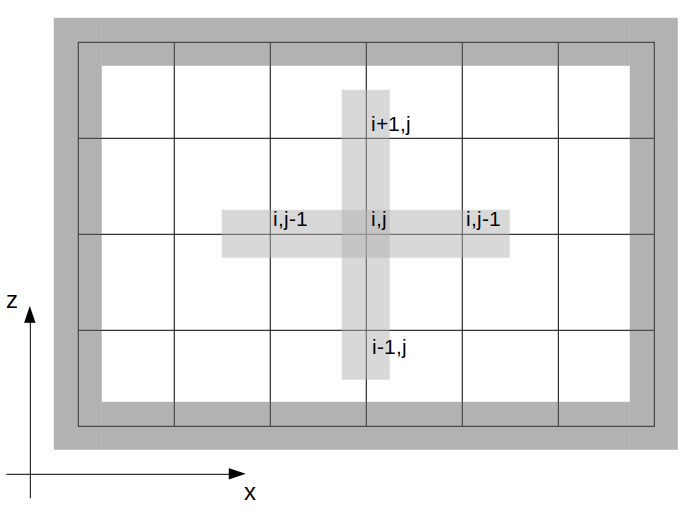
\includegraphics[width=\linewidth]{2d-grid}
\caption{Finite difference discretization of the 2D heat problem}
\label{fig:2d-grid}
\end{figure}

According to the previous explanation on Taylor-series expansion and Linearization of PDEs, if we employ a fully implicit, unconditionally stable discretization scheme as we have done for the 1D equation , equation \ref{eq:2DheatOtherForm} can be written as

\begin{equation}
\frac{\phi^{n+1}_{i,j}-\phi^{n}_{i,j}}{\Delta t} = D ( \frac{\phi^{n+1}_{i,j+1}-2\phi^{n+1}_{i,j}+\phi^{n+1}_{i,j-1}}{(\Delta x)^2} + \frac{\phi^{n+1}_{i+1,j}-2\phi^{n+1}_{i,j}+\phi^{n+1}_{i-1,j}}{(\Delta z)^2} )
\end{equation}
Rearranging terms with $n + 1$ on one side and terms with $n$ on the other side gives
\begin{equation}
\phi^{n}_{i,j} =-s_z \phi^{n+1}_{i+1,j}-s_x \phi^{n+1}_{i,j+1} +(1+2s_z+2s_x) \phi^{n+1}_{i,j} -s_z \phi^{n+1}_{i-1,j}-s_x \phi^{n+1}_{i,j-1}
\label{eq:2Ddescrete}
\end{equation}
As in the 1D case, we have to write these equations in a matrix $A$ and a vector $\vec{b}$. From a practical point of view, this is a bit more complicated than in the 1D case, since we have to deal with “book-keeping” issues, i.e. the mapping of $\phi_{i,j}$ to the entries of a vector $\Phi_k$. 
\\
If a 2D scalar field is to be solved for with an equivalent vector $\Phi$, the nodes have to be numbered continuously, for example as in Figure \ref{fig:2d-grid-mapping}. The derivative versus x-direction is then e.g.

\begin{figure}[ht]\centering
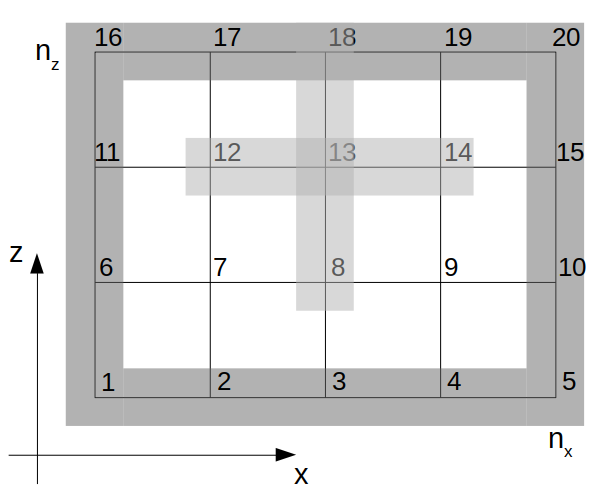
\includegraphics[width=\linewidth]{2d-grid-mapping}
\caption{Numbering scheme for a 2D grid with $n_x = 5$ and $n_z = 4$.}
\label{fig:2d-grid-mapping}
\end{figure}

\begin{equation}
\frac{\partial^2 \phi}{\partial x^2}|_{i=3,j=3}= \frac{1}{(\Delta x)^2}(\Phi_{14}-2\Phi_{13}+\Phi_{12})
\label{eq:grid19x}
\end{equation}
and the derivative versus z-direction is given by
\begin{equation}
\frac{\partial^2 \phi}{\partial z^2}|_{i=3,j=3}= \frac{1}{(\Delta z)^2}(\Phi_{18}-2\Phi_{13}+\Phi_{8})
\label{eq:grid19z}
\end{equation}

If $n_x$ are the number of grid points in x-direction and $n_z$ the number of points in z-direction, we can write equations \ref{eq:grid19x} and \ref{eq:grid19z} in a more general way as:
\begin{equation}
\frac{\partial^2 \phi}{\partial x^2}|_{i,j}= \frac{1}{(\Delta x)^2}(\phi_{(i-1)n_x+j+1}-2\phi_{(i-1)n_x+j}+\phi_{(i-1)n_x+j-1})
\label{eq:gridKx}
\end{equation}
\begin{equation}
\frac{\partial^2 \phi}{\partial z^2}|_{i,j}= \frac{1}{(\Delta z)^2}(\phi_{in_x+j}-2\phi_{(i-1)n_x+j}+\phi_{(i-2)n_x+j})
\label{eq:gridKz}
\end{equation}

As an example, for a $4 \times 5$ grid there are $20$ grid points but $14$ of them are boundary points (located at left, right, top, and bottom) which do not have evolution. There are only $6$ middle points that have evolution in time. Thus, the coefficint matrix $A$ is $20 \times 20$, and on $14$ rows we have just one non-zero element (corresponding to the boundary condition).
\\
According to equation \ref{eq:2Ddescrete}, for a $4 \times 5$ grid, for example, at the boundary points the linear system becomes
%\begin{equation}
\begin{align}
bottom &: \qquad \phi^{n+1}_{1,1}= \phi^{n+1}_{1,2}=\phi^{n+1}_{1,3}=\phi^{n+1}_{1,4}=\phi^{n+1}_{1,5}=\phi_{bottom} \\
top &: \qquad \phi^{n+1}_{4,1}=\phi^{n+1}_{4,2}=\phi^{n+1}_{4,3}=\phi^{n+1}_{4,4}=\phi^{n+1}_{4,5} = \phi_{top} \\
left &: \qquad \phi^{n+1}_{2,1}=\phi^{n+1}_{3,1}=\phi_{left} \\
right &: \qquad \phi^{n+1}_{2,5}=\phi^{n+1}_{3,5}= \phi_{right} \\
\label{eq:2D45boundary}
\end{align}
%\end{equation}
\begin{align}
grid \ point \ 2,2 &:-s_z \phi^{n+1}_{3,2} -s_x \phi^{n+1}_{2,3} +(1+s_z+s_x) \phi^{n+1}_{2,2} -s_z \phi^{n+1}_{1,2} -s_x \phi^{n+1}_{2,1}  = \phi^{n+1}_{2,2} \\
grid \ point \ 2,3 &:-s_z \phi^{n+1}_{3,3} -s_x \phi^{n+1}_{2,4} +(1+s_z+s_x) \phi^{n+1}_{2,3} -s_z \phi^{n+1}_{1,3} -s_x \phi^{n+1}_{2,2}  = \phi^{n+1}_{2,3} \\
grid \ point \  2,4 &:-s_z \phi^{n+1}_{3,5} -s_x \phi^{n+1}_{2,5} +(1+s_z+s_x) \phi^{n+1}_{2,4} -s_z \phi^{n+1}_{1,4} -s_x \phi^{n+1}_{2,3}  = \phi^{n+1}_{2,4} \\
grid \ point \ 3,2 &:-s_z \phi^{n+1}_{4,2} -s_x \phi^{n+1}_{3,3} +(1+s_z+s_x) \phi^{n+1}_{3,2} -s_z \phi^{n+1}_{2,2} -s_x \phi^{n+1}_{3,1}  = \phi^{n+1}_{3,2} \\
grid \ point \ 3,3 &:-s_z \phi^{n+1}_{4,3} -s_x \phi^{n+1}_{3,4} +(1+s_z+s_x) \phi^{n+1}_{3,3} -s_z \phi^{n+1}_{2,3} -s_x \phi^{n+1}_{3,2}  = \phi^{n+1}_{3,3} \\
grid \ point \ 3,4 &:-s_z \phi^{n+1}_{4,4} -s_x \phi^{n+1}_{3,5} +(1+s_z+s_x) \phi^{n+1}_{3,4} -s_z \phi^{n+1}_{2,4} -s_x \phi^{n+1}_{3,3}  = \phi^{n+1}_{3,4} \\
\label{eq:2D45middle}
\end{align}
%\end{equation}
%\end{table*}


and the linear system for the $6$ other points located between the boundaries becomes \ref{eq:2D45middle}.  
\\

%\begin{table*}[ht]
%\begin{equation}

As we explained previously the “book-keeping” issues, i.e. the mapping of $\phi_{i,j}$ to the vector $\Phi_k$ , vectors $\vec{x}$ and $\vec{b}$ become equation \ref{eq:2D45xb}.

\begin{equation}
x= \begin{bmatrix}
	\phi^{n+1}_{1,1} \\ \phi^{n+1}_{1,2} \\ \phi^{n+1}_{1,3} \\ \phi^{n+1}_{1,4} \\ \phi^{n+1}_{1,5} \\ \phi^{n+1}_{2,1} \\ \phi^{n+1}_{2,2} \\ \phi^{n+1}_{2,3} \\ \phi^{n+1}_{2,4} \\ \phi^{n+1}_{2,5} \\ \phi^{n+1}_{3,1} \\ \phi^{n+1}_{3,2} \\ \phi^{n+1}_{3,3} \\ \phi^{n+1}_{3,4} \\ \phi^{n+1}_{3,5} \\ \phi^{n+1}_{4,1} \\ \phi^{n+1}_{4,2} \\ \phi^{n+1}_{4,3} \\ \phi^{n+1}_{4,4} \\ \phi^{n+1}_{4,5} 
\end{bmatrix}
=
   \begin{bmatrix}
	\Phi^{n+1}_{1} \\ \Phi^{n+1}_{2} \\ \Phi^{n+1}_{3} \\ \Phi^{n+1}_{4} \\ \Phi^{n+1}_{5} \\ \Phi^{n+1}_{6} \\ \Phi^{n+1}_{7} \\ \Phi^{n+1}_{8} \\ \Phi^{n+1}_{9} \\ \Phi^{n+1}_{10} \\ \Phi^{n+1}_{11} \\ \Phi^{n+1}_{12} \\ \Phi^{n+1}_{13} \\ \Phi^{n+1}_{14} \\ \Phi^{n+1}_{15} \\ \Phi^{n+1}_{16} \\ \Phi^{n+1}_{17} \\ \Phi^{n+1}_{18} \\ \Phi^{n+1}_{19} \\ \Phi^{n+1}_{20} 
   \end{bmatrix}
    , \qquad \quad
b= \begin{bmatrix}
	\phi^{n}_{1,1} \\ \phi^{n}_{1,2} \\ \phi^{n}_{1,3} \\ \phi^{n}_{1,4} \\ \phi^{n}_{1,5} \\ \phi^{n}_{2,1} \\ \phi^{n}_{2,2} \\ \phi^{n}_{2,3} \\ \phi^{n}_{2,4} \\ \phi^{n}_{2,5} \\ \phi^{n}_{3,1} \\ \phi^{n}_{3,2} \\ \phi^{n}_{3,3} \\ \phi^{n}_{3,4} \\ \phi^{n}_{3,5} \\ \phi^{n}_{4,1} \\ \phi^{n}_{4,2} \\ \phi^{n}_{4,3} \\ \phi^{n}_{4,4} \\ \phi^{n}_{4,5} 
\end{bmatrix}
=
\begin{bmatrix}
	\phi_{bottom} \\ \phi_{bottom} \\ \phi_{bottom} \\ \phi_{bottom} \\ \phi_{bottom} \\ \phi_{left} \\ \Phi^{n}_{7} \\ \Phi^{n}_{8} \\ \Phi^{n}_{9} \\ \phi_{right} \\ \phi_{left} \\ \Phi^{n}_{12} \\ \Phi^{n}_{13} \\ \Phi^{n}_{14} \\ \phi_{right} \\ \phi_{top} \\ \phi_{top} \\ \phi_{top} \\ \phi_{top} \\ \phi_{top} 
\end{bmatrix}
\label{eq:2D45xb}
\end{equation}
And the coefficient matrix, $A$, is \ref{eq:2D45A}. 
\\ 
Now two-dimentional heat equation (\ref{eq:2Dheat}) on a $5 \times 4$ grid reduced to a linear system $A\vec{x}=\vec{b}$, with  $\vec{x}$, $\vec{b}$, and $A$ are given by equations \ref{eq:2D45xb}, \ref{eq:2D45A}. 
\\
This is the way to find the coefficient matrix, and notice that for different boundary conditions we should modify some elements in the coefficient matrix. You can easily understand the pattern in the coefficient matrix, it will help you to build it in your code.
\\
Now that we know how to build the coefficient matrix for two-dimentional problem, it is the time to check what we have orgnized so far. 

\pagebreak

%\afterpage{%
%    \clearpage% Flush earlier floats (otherwise order might not be correct)
%    \thispagestyle{empty}% empty page style (?)
    \begin{landscape}% Landscape page
 	The coefficient matrix, $A$, for a $5 \times 4$ grid is
%\begin{flushleft}
 %   Thus the coefficient matrix, $A$, is
%\end{flushleft}
        \centering % Center table
\begin{equation}
\setcounter{MaxMatrixCols}{20}
\footnotesize{
A = \begin{bmatrix}
    \begin{array}{ccccc|ccccc|ccccc|ccccc}
       1 & 0 & 0 & 0 & 0 & 0 & 0 & 0 & 0 & 0 & 0 & 0 & 0 & 0 & 0 & 0 & 0 & 0 & 0 & 0 \\ %1
       0 & 1 & 0 & 0 & 0 & 0 & 0 & 0 & 0 & 0 & 0 & 0 & 0 & 0 & 0 & 0 & 0 & 0 & 0 & 0 \\ %2
       0 & 0 & 1 & 0 & 0 & 0 & 0 & 0 & 0 & 0 & 0 & 0 & 0 & 0 & 0 & 0 & 0 & 0 & 0 & 0 \\ %3
       0 & 0 & 0 & 1 & 0 & 0 & 0 & 0 & 0 & 0 & 0 & 0 & 0 & 0 & 0 & 0 & 0 & 0 & 0 & 0 \\ %4
       0 & 0 & 0 & 0 & 1 & 0 & 0 & 0 & 0 & 0 & 0 & 0 & 0 & 0 & 0 & 0 & 0 & 0 & 0 & 0 \\ %5
         \hline
       0 & 0 & 0 & 0 & 0 & 1 & 0 & 0 & 0 & 0 & 0 & 0 & 0 & 0 & 0 & 0 & 0 & 0 & 0 & 0 \\ %6
       0 & -s_z & 0 & 0 & 0 & -s_x & (1+2s_z+2s_x) & -s_x & 0 & 0 & 0 & -s_z & 0 & 0 & 0 & 0 & 0 & 0 & 0 & 0 \\ %7
       0 & 0 & -s_z & 0 & 0 & 0 & -s_x & 1+2s_z+2s_x & -s_x & 0 & 0 & 0 & -s_z & 0 & 0 & 0 & 0 & 0 & 0 & 0 \\ %8
       0 & 0 & 0 & -s_z & 0 & 0 & 0 & -s_x & 1+2s_z+2s_x & -s_x & 0 & 0 & 0 & -s_z & 0 & 0 & 0 & 0 & 0 & 0 \\ %9
       0 & 0 & 0 & 0 & 0 & 0 & 0 & 0 & 0 & 1 & 0 & 0 & 0 & 0 & 0 & 0 & 0 & 0 & 0 & 0 \\ %10
          \hline
       0 & 0 & 0 & 0 & 0 & 0 & 0 & 0 & 0 & 0 & 1 & 0 & 0 & 0 & 0 & 0 & 0 & 0 & 0 & 0 \\ %11
       0 & 0 & 0 & 0 & 0 & 0 & -s_z & 0 & 0 & 0 & -s_x & 1+2s_z+2s_x & -s_x & 0 & 0 & 0 & -s_z & 0 & 0 & 0 \\ %12
       0 & 0 & 0 & 0 & 0 & 0 & 0 & -s_z & 0 & 0 & 0 & -s_x & 1+2s_z+2s_x & -s_x & 0 & 0 & 0 & -s_z & 0 & 0 \\ %13
       0 & 0 & 0 & 0 & 0 & 0 & 0 & 0 & -s_z & 0 & 0 & 0 & -s_x & 1+2s_z+2s_x & -s_x & 0 & 0 & 0 & -s_z & 0 \\ %14
       0 & 0 & 0 & 0 & 0 & 0 & 0 & 0 & 0 & 0 & 0 & 0 & 0 & 0 & 1 & 0 & 0 & 0 & 0 & 0 \\ %15
         \hline
       0 & 0 & 0 & 0 & 0 & 0 & 0 & 0 & 0 & 0 & 0 & 0 & 0 & 0 & 0 & 1 & 0 & 0 & 0 & 0 \\ %16
       0 & 0 & 0 & 0 & 0 & 0 & 0 & 0 & 0 & 0 & 0 & 0 & 0 & 0 & 0 & 0 & 1 & 0 & 0 & 0 \\ %17
       0 & 0 & 0 & 0 & 0 & 0 & 0 & 0 & 0 & 0 & 0 & 0 & 0 & 0 & 0 & 0 & 0 & 1 & 0 & 0 \\ %18
       0 & 0 & 0 & 0 & 0 & 0 & 0 & 0 & 0 & 0 & 0 & 0 & 0 & 0 & 0 & 0 & 0 & 0 & 1 & 0 \\ %19
       0 & 0 & 0 & 0 & 0 & 0 & 0 & 0 & 0 & 0 & 0 & 0 & 0 & 0 & 0 & 0 & 0 & 0 & 0 & 1 \\ %20
   \end{array}
    \end{bmatrix}
\label{eq:2D45A}
}
\end{equation}

 	The coefficient matrix, $A$, for a $4 \times 5$ grid is
%inja
\begin{equation}
\setcounter{MaxMatrixCols}{20}
\footnotesize{
A = \begin{bmatrix}
    \begin{array}{cccc|cccc|cccc|cccc|cccc}
       1 & 0 & 0 & 0 & 0 & 0 & 0 & 0 & 0 & 0 & 0 & 0 & 0 & 0 & 0 & 0 & 0 & 0 & 0 & 0 \\ %1
       0 & 1 & 0 & 0 & 0 & 0 & 0 & 0 & 0 & 0 & 0 & 0 & 0 & 0 & 0 & 0 & 0 & 0 & 0 & 0 \\ %2
       0 & 0 & 1 & 0 & 0 & 0 & 0 & 0 & 0 & 0 & 0 & 0 & 0 & 0 & 0 & 0 & 0 & 0 & 0 & 0 \\ %3
       0 & 0 & 0 & 1 & 0 & 0 & 0 & 0 & 0 & 0 & 0 & 0 & 0 & 0 & 0 & 0 & 0 & 0 & 0 & 0 \\ %4
         \hline
       0 & 0 & 0 & 0 & 1 & 0 & 0 & 0 & 0 & 0 & 0 & 0 & 0 & 0 & 0 & 0 & 0 & 0 & 0 & 0 \\ %5
       0 & -s_z & 0 & 0 & -s_x & 1+2s_z+2s_x & -s_x & 0 & 0 & -s_z & 0 & 0 & 0 & 0 & 0 & 0 & 0 & 0 & 0 & 0 \\ %6
       0 & 0 & -s_z & 0 & 0 & -s_x & 1+2s_z+2s_x & -s_x & 0 & 0 & -s_z & 0 & 0 & 0 & 0 & 0 & 0 & 0 & 0 & 0 \\ %7
       0 & 0 & 0 & 0 & 0 & 0 & 0 & 1 & 0 & 0 & 0 & 0 & 0 & 0 & 0 & 0 & 0 & 0 & 0 & 0 \\ %8
       \hline
       0 & 0 & 0 & 0 & 0 & 0 & 0 & 0 & 1 & 0 & 0 & 0 & 0 & 0 & 0 & 0 & 0 & 0 & 0 & 0 \\ %9
       0 & 0 & 0 & 0 & 0 & -s_z & 0 & 0 & -s_x & 1+2s_z+2s_x & -s_x & 0 & 0 & -s_z & 0 & 0 & 0 & 0 & 0 & 0 \\ %10
       0 & 0 & 0 & 0 & 0 & 0 & -s_z & 0 & 0 & -s_x & 1+2s_z+2s_x & -s_x & 0 & 0 & -s_z & 0 & 0 & 0 & 0 & 0 \\ %11
       0 & 0 & 0 & 0 & 0 & 0 & 0 & 0 & 0 & 0 & 0 & 1 & 0 & 0 & 0 & 0 & 0 & 0 & 0 & 0 \\ %12
       \hline
       0 & 0 & 0 & 0 & 0 & 0 & 0 & 0 & 0 & 0 & 0 & 0 & 1 & 0 & 0 & 0 & 0 & 0 & 0 & 0 \\ %13
       0 & 0 & 0 & 0 & 0 & 0 & 0 & 0 & 0 & -s_z & 0 & 0 & -s_x & 1+2s_z+2s_x & -s_x & 0 & 0 & -s_z & 0 & 0 \\ %14
       0 & 0 & 0 & 0 & 0 & 0 & 0 & 0 & 0 & 0 & -s_z & 0 & 0 & -s_x & 1+2s_z+2s_x & -s_x & 0 & 0 & -s_z & 0 \\ %15
       0 & 0 & 0 & 0 & 0 & 0 & 0 & 0 & 0 & 0 & 0 & 0 & 0 & 0 & 0 & 1 & 0 & 0 & 0 & 0 \\ %16
       \hline
       0 & 0 & 0 & 0 & 0 & 0 & 0 & 0 & 0 & 0 & 0 & 0 & 0 & 0 & 0 & 0 & 1 & 0 & 0 & 0 \\ %17
       0 & 0 & 0 & 0 & 0 & 0 & 0 & 0 & 0 & 0 & 0 & 0 & 0 & 0 & 0 & 0 & 0 & 1 & 0 & 0 \\ %18
       0 & 0 & 0 & 0 & 0 & 0 & 0 & 0 & 0 & 0 & 0 & 0 & 0 & 0 & 0 & 0 & 0 & 0 & 1 & 0 \\ %19
       0 & 0 & 0 & 0 & 0 & 0 & 0 & 0 & 0 & 0 & 0 & 0 & 0 & 0 & 0 & 0 & 0 & 0 & 0 & 1 \\ %20
   \end{array}
    \end{bmatrix}
\label{eq:2D54A}
}
\end{equation}

\end{landscape}



Like what we have done for the one-dimentional part, here we can ignore the boundary points in the solution vector (all $\phi_{top}$, $\phi_{bottom}$, $\phi_{left}$, and $\phi{right}$) and just solve the equation for the evolving middle ponits. Like befor we consider the boundary conditions in a boundary condition vector ($\vec{b.c.}$). For two dimensional case, we can rewrite the linear system as:
\begin{equation}
A'\vec{x'}=\vec{b}+\vec{b.c.}
\end{equation} 
where vectors $\vec{x'}$, $\vec{b'}$, and $\vec{b.c.}$ are:
\begin{equation}
\vec{x'}=\begin{bmatrix}
 \Phi^{n+1}_{7} \\ \Phi^{n+1}_{8} \\ \Phi^{n+1}_{9} \\  \Phi^{n+1}_{12} \\ \Phi^{n+1}_{13} \\ \Phi^{n+1}_{14}
\end{bmatrix}
\quad
\vec{b'}=\begin{bmatrix}
 \Phi^{n}_{7} \\ \Phi^{n}_{8} \\ \Phi^{n}_{9} \\  \Phi^{n}_{12} \\ \Phi^{n}_{13} \\ \Phi^{n}_{14}
\end{bmatrix}
\quad
\vec{b.c.}= \begin{bmatrix}
+s_{z} \phi_{bottom} +s_{x} \phi_{left} \\ +s_{z} \phi_{bottom} \\ +s_{z} \phi_{bottom} + s_{x} \phi_{right}  \\ +s_{z} \phi_{top} + s_{x} \phi_{left} \\ +s_{z} \phi_{top} \\ +s_{z} \phi_{top} + s_{x} \phi_{right}
\end{bmatrix}
\end{equation}
and coefficient matrix $A'$ is \ref{eq:coefmatrix2dA'}

\begin{table*}[ht]
\begin{equation}
A' = \begin{bmatrix}
	   (1+2s_z +2 s_x) & -s_x & 0 & -s_z & 0 & 0  \\
   	   -s_x & (1+2s_z +2 s_x) &-s_x & 0 & -s_z & 0   \\
   	   0 & -s_x & (1+2s_z +2 s_x) &-s_x & 0 & -s_z   \\
  	   -s_z & 0 & -s_x & (1+2s_z +2 s_x) &-s_x & 0   \\
   	   0 & -s_z & 0 & -s_x & (1+2s_z +2 s_x) &-s_x  \\
   	   0 & 0 & -s_z & 0 & -s_x & (1+2s_z +2 s_x)  \\
     \end{bmatrix}
     \label{eq:coefmatrix2dA'}
\end{equation}
\end{table*}



\section{Results for two-dimensional heat equation}
\subsection{The case of constant diffusion coefficient}
In the previous sections we have found that the CG algorithm are much more efficient than the direct methods such as LU decomposition, so all the simulation for the two-dimentional equation have been done using CG method.
\\
\begin{figure}[ht]\centering
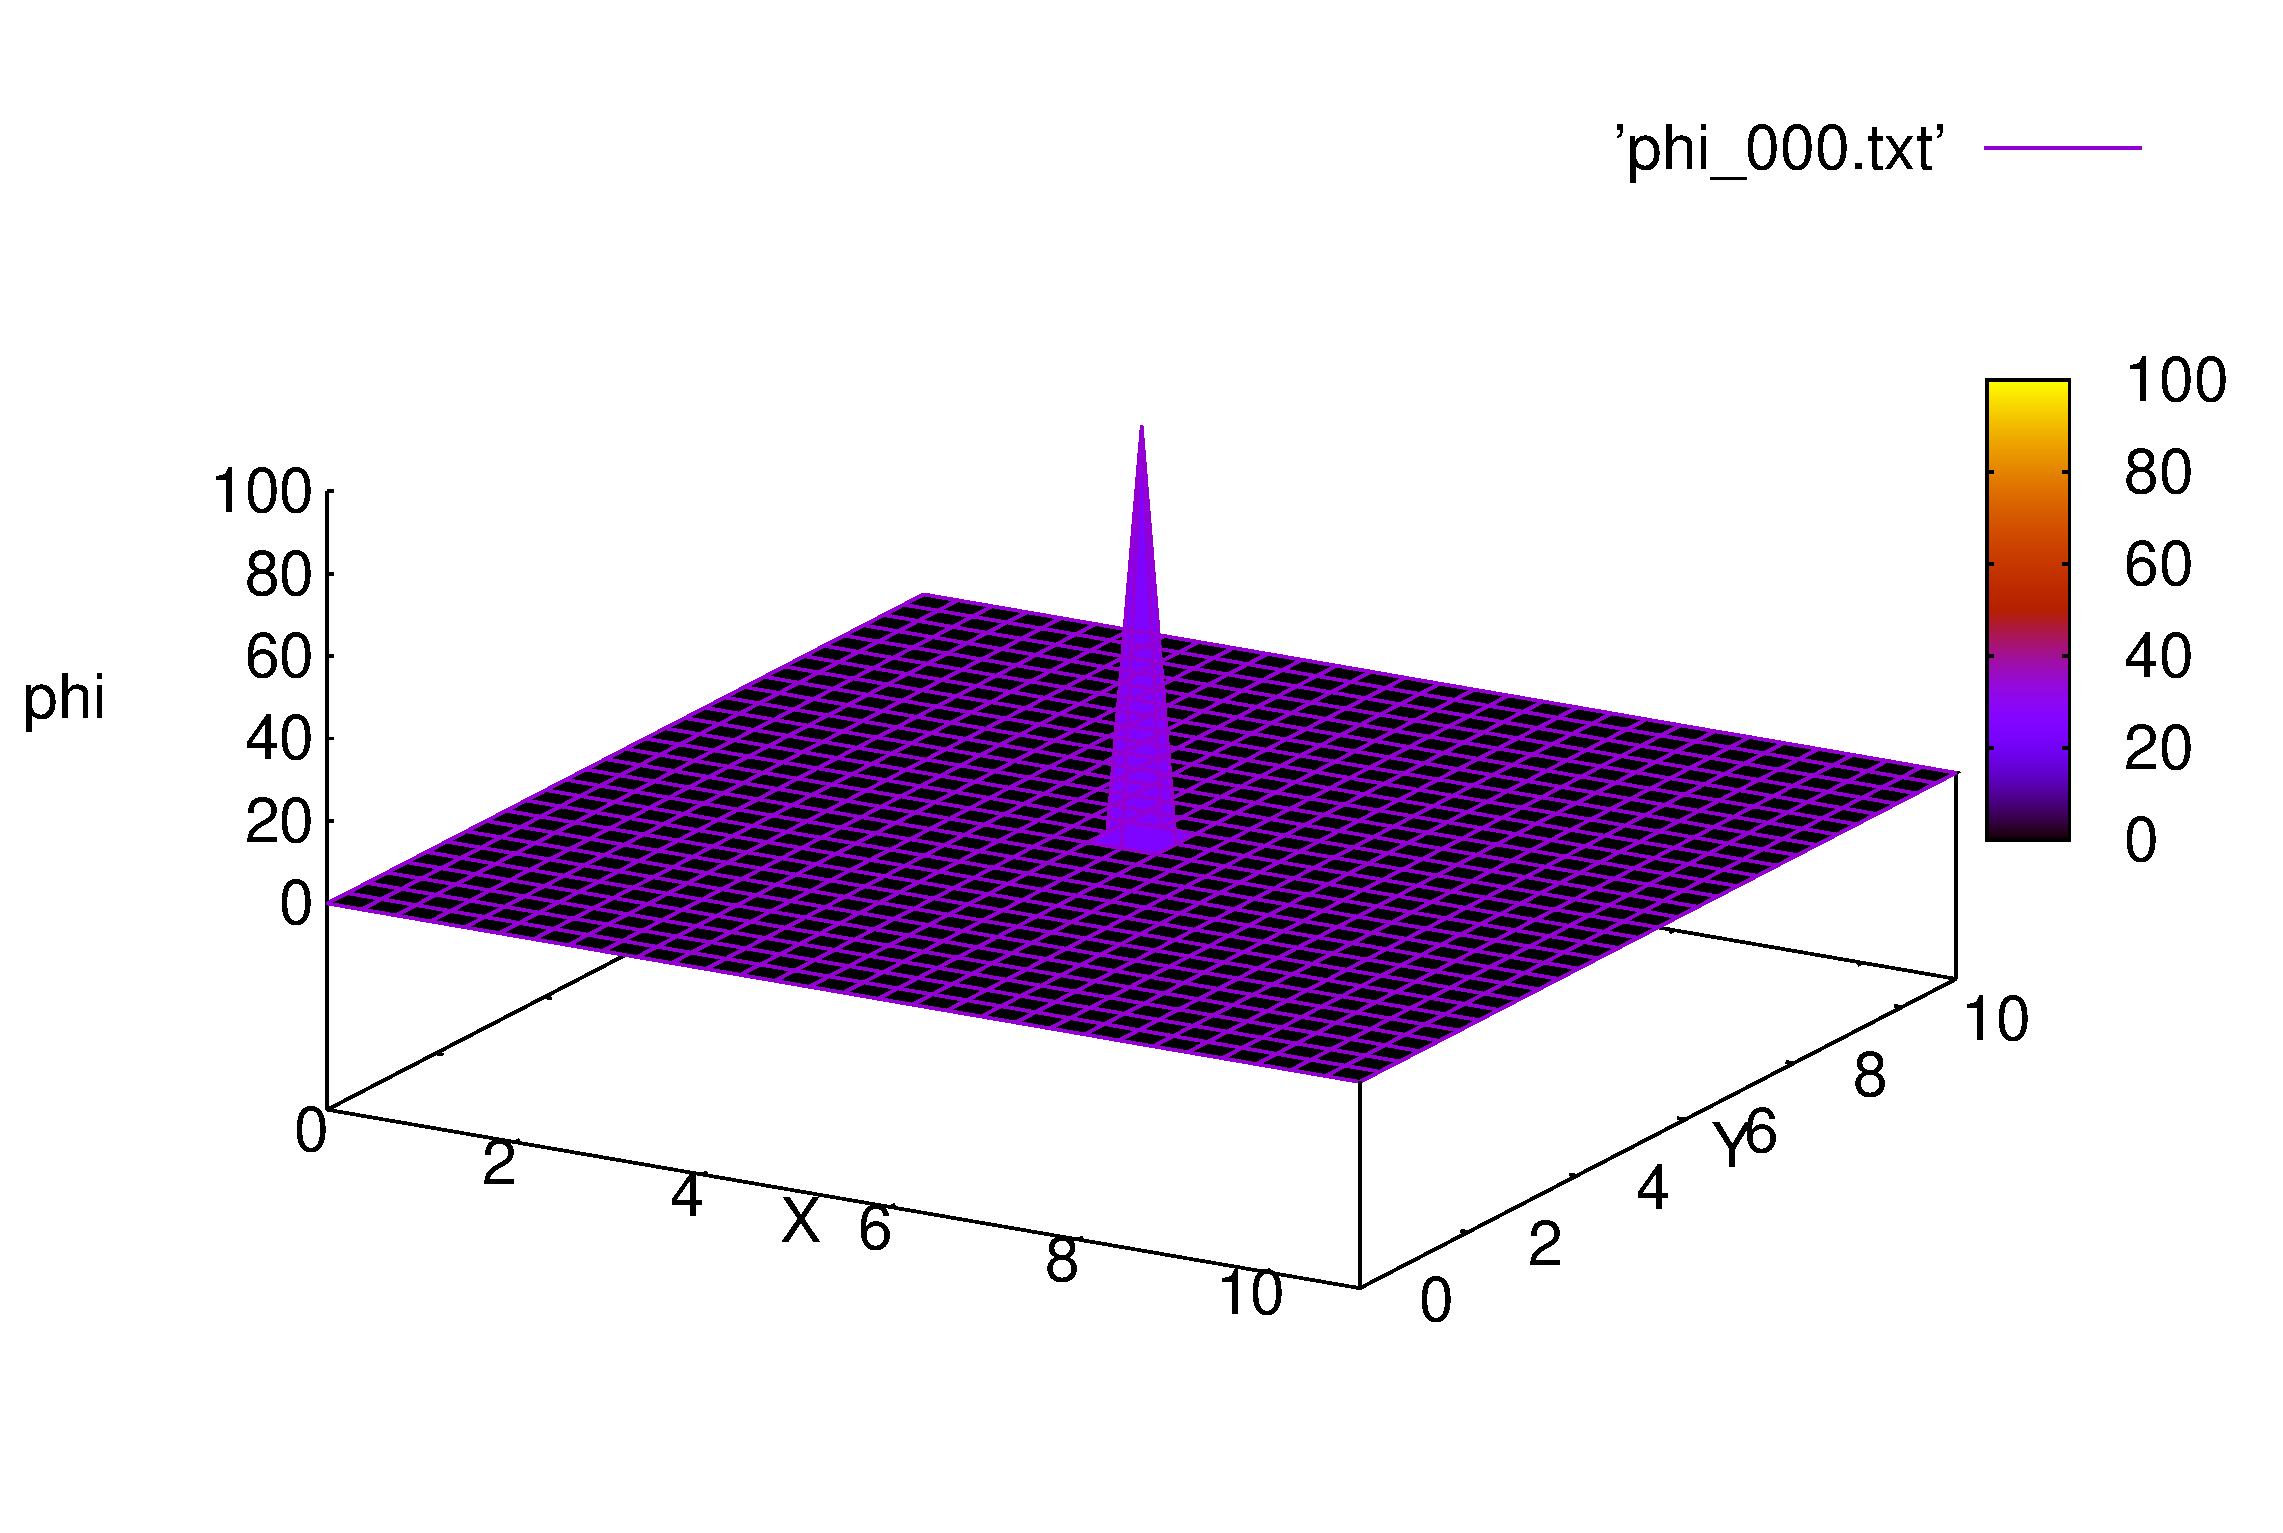
\includegraphics[width=\linewidth]{2DSimplefig/00}
\caption{initial condition for the 2D heat problem}
\label{fig:2d-initial_condition}
\end{figure}


%For the next step you will get figure \ref{fig:2d-1dt}.

%\begin{figure}[ht]\centering
%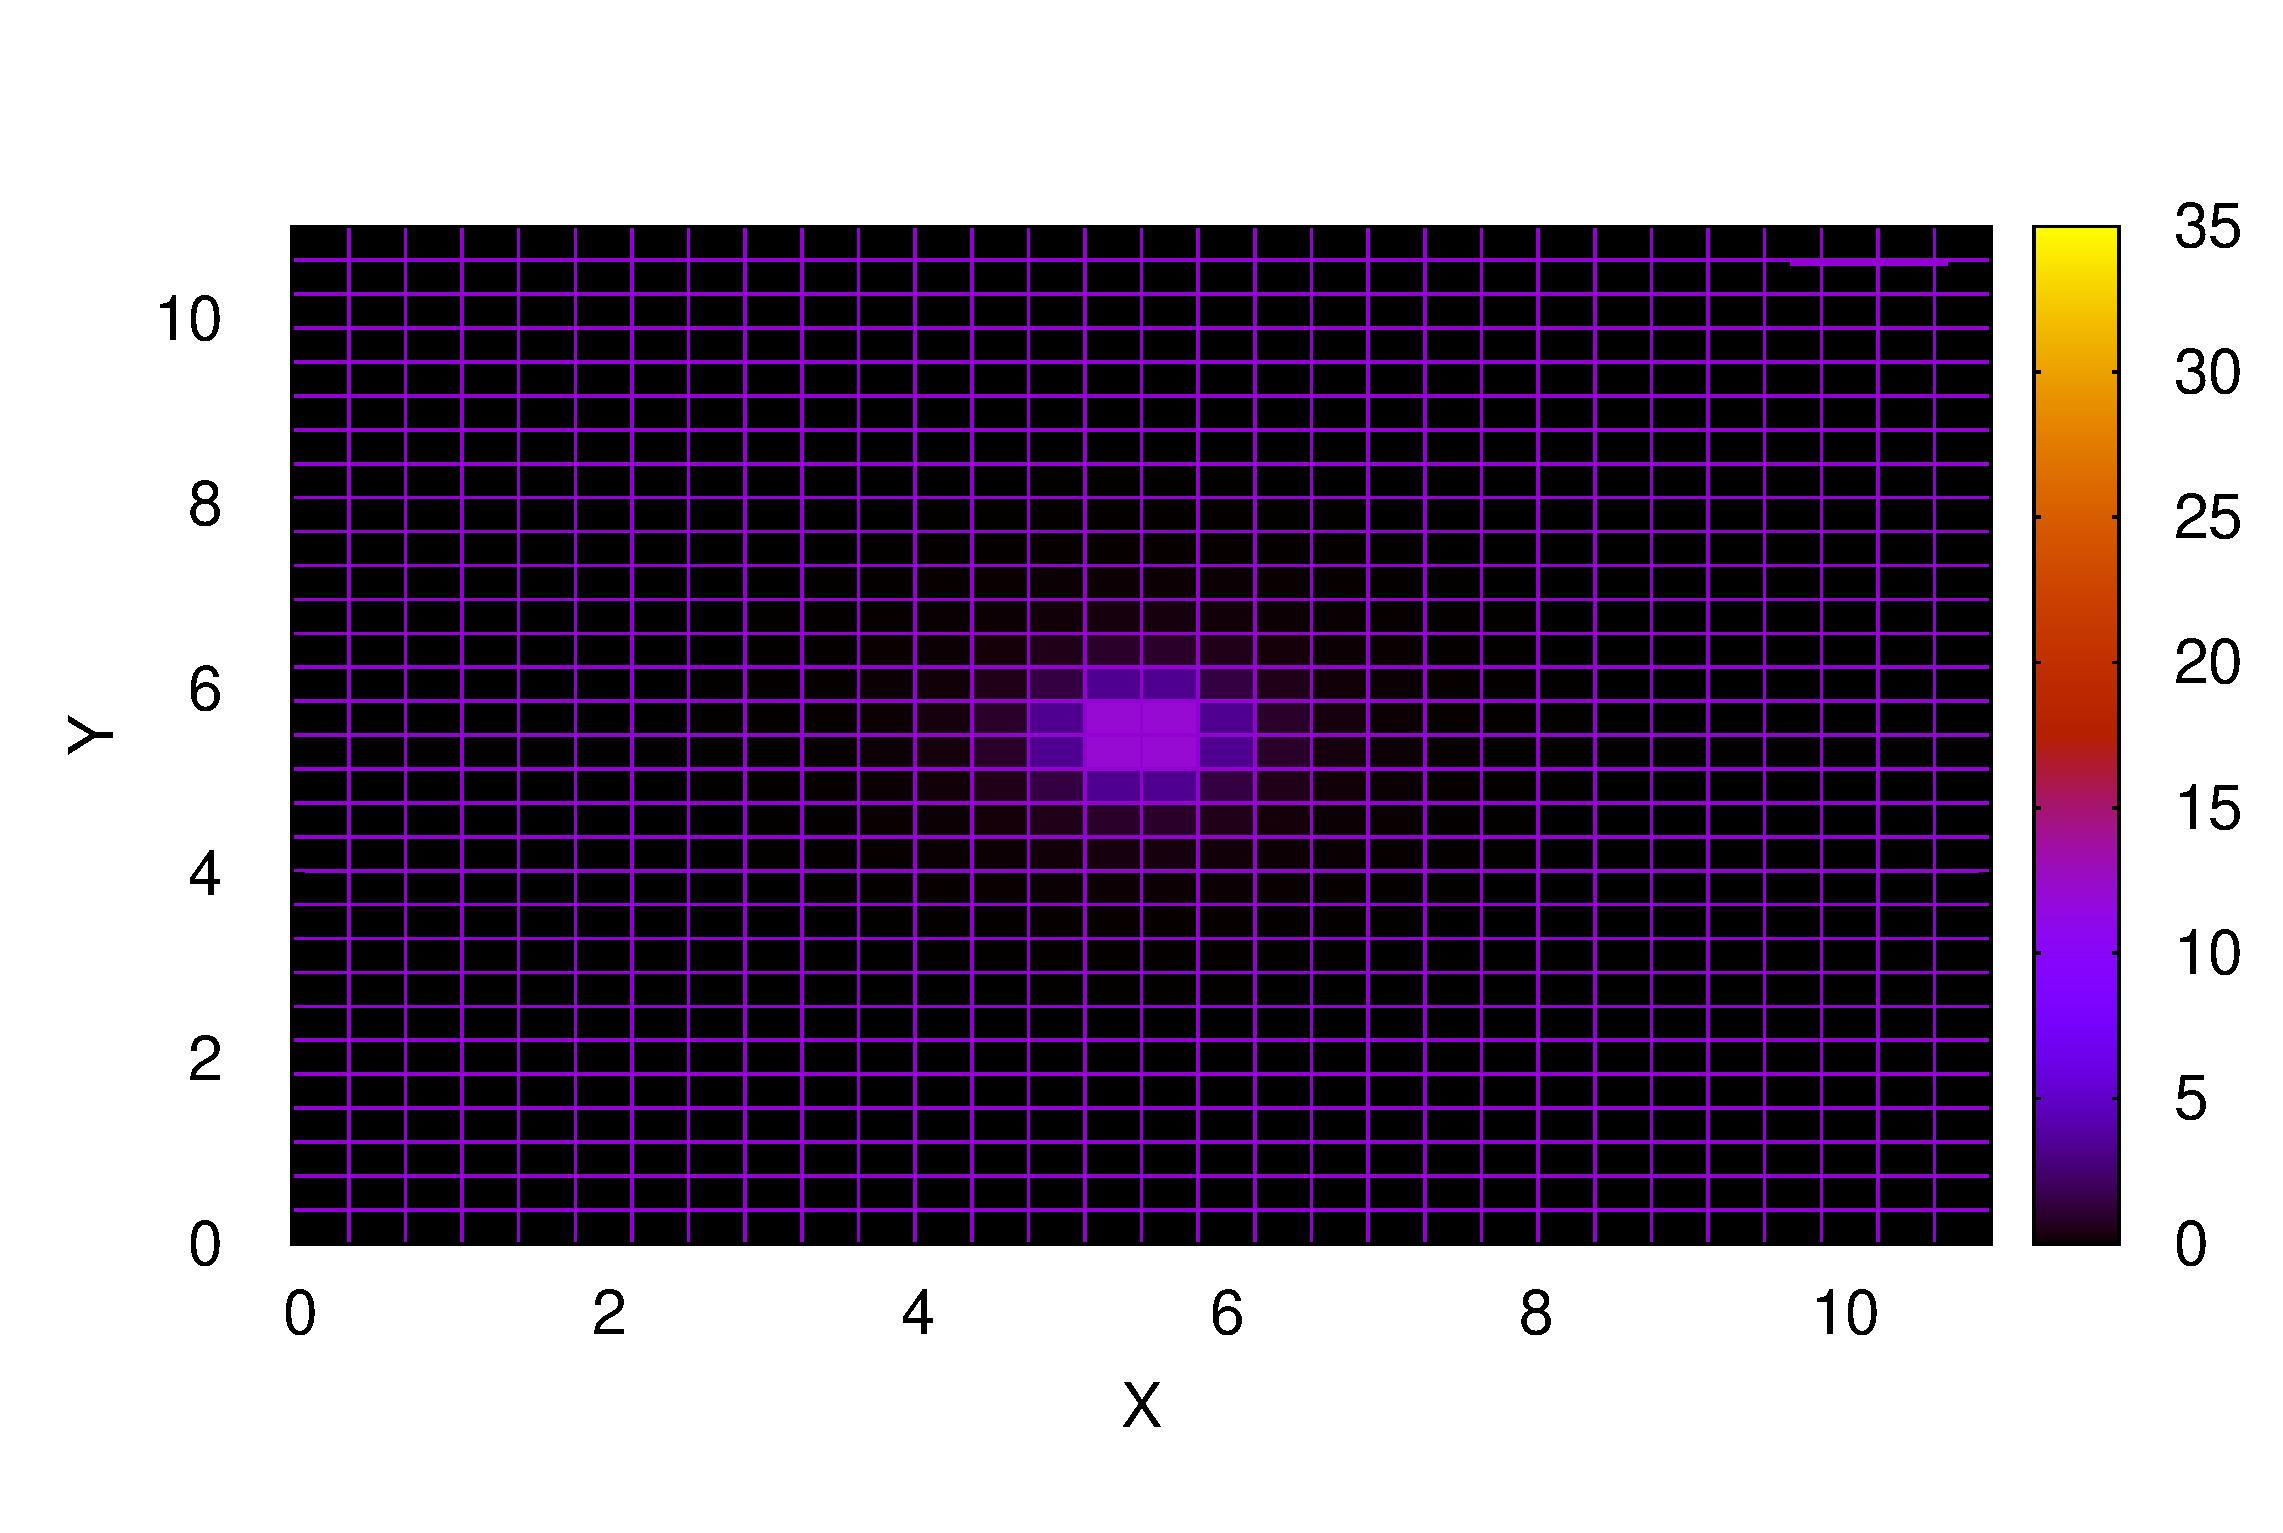
\includegraphics[width=\linewidth]{2DSimplefig/01_map}
%\caption{First step for the 2D heat problem}
%\label{fig:2d-1dt}
%\end{figure}

After 10 steps we will have figure \ref{fig:2d-10dt}. There is also an animation accessible at: \\
  \texttt{http://www.github.com/}. \\


\begin{figure}
     \centering
     \begin{subfigure}[b]{0.5\textwidth}
         \centering
         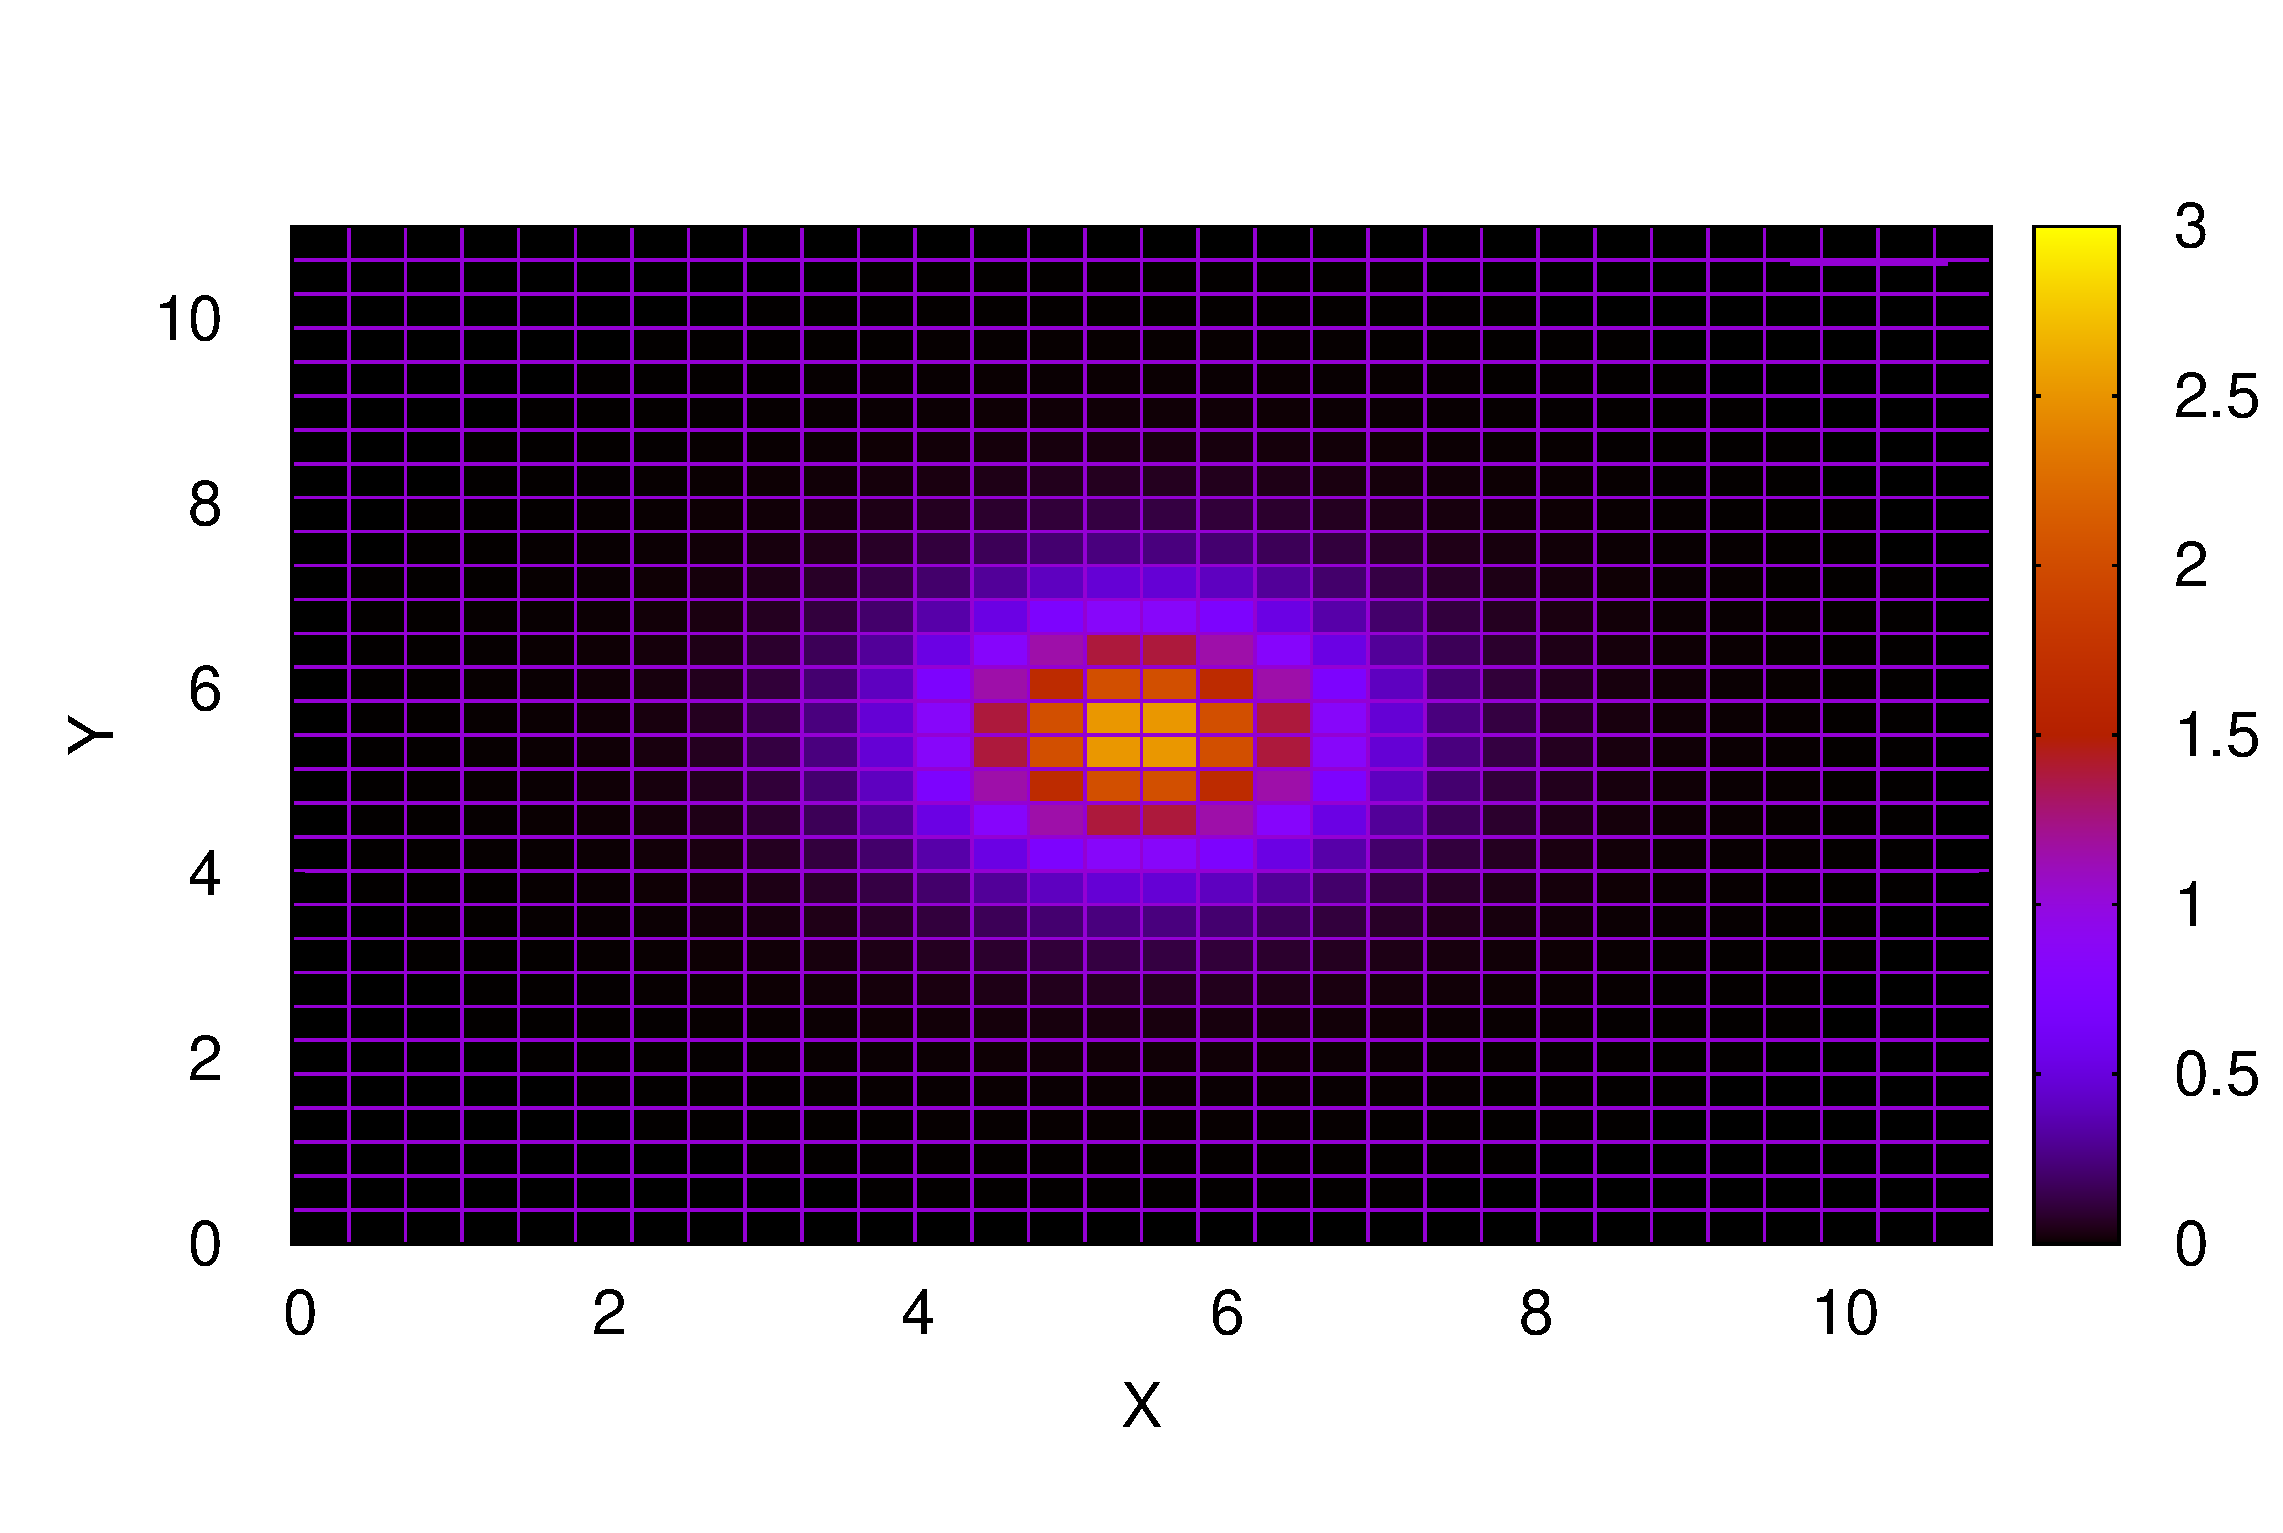
\includegraphics[width=\textwidth]{2DSimplefig/05_map}
		\caption{the heat distribution map after 5 timesteps for the 2D heat problem}
		\label{fig:2d-5dt}
     \end{subfigure}
     \hfill
	\centering
     \begin{subfigure}[b]{0.5\textwidth}
         \centering
         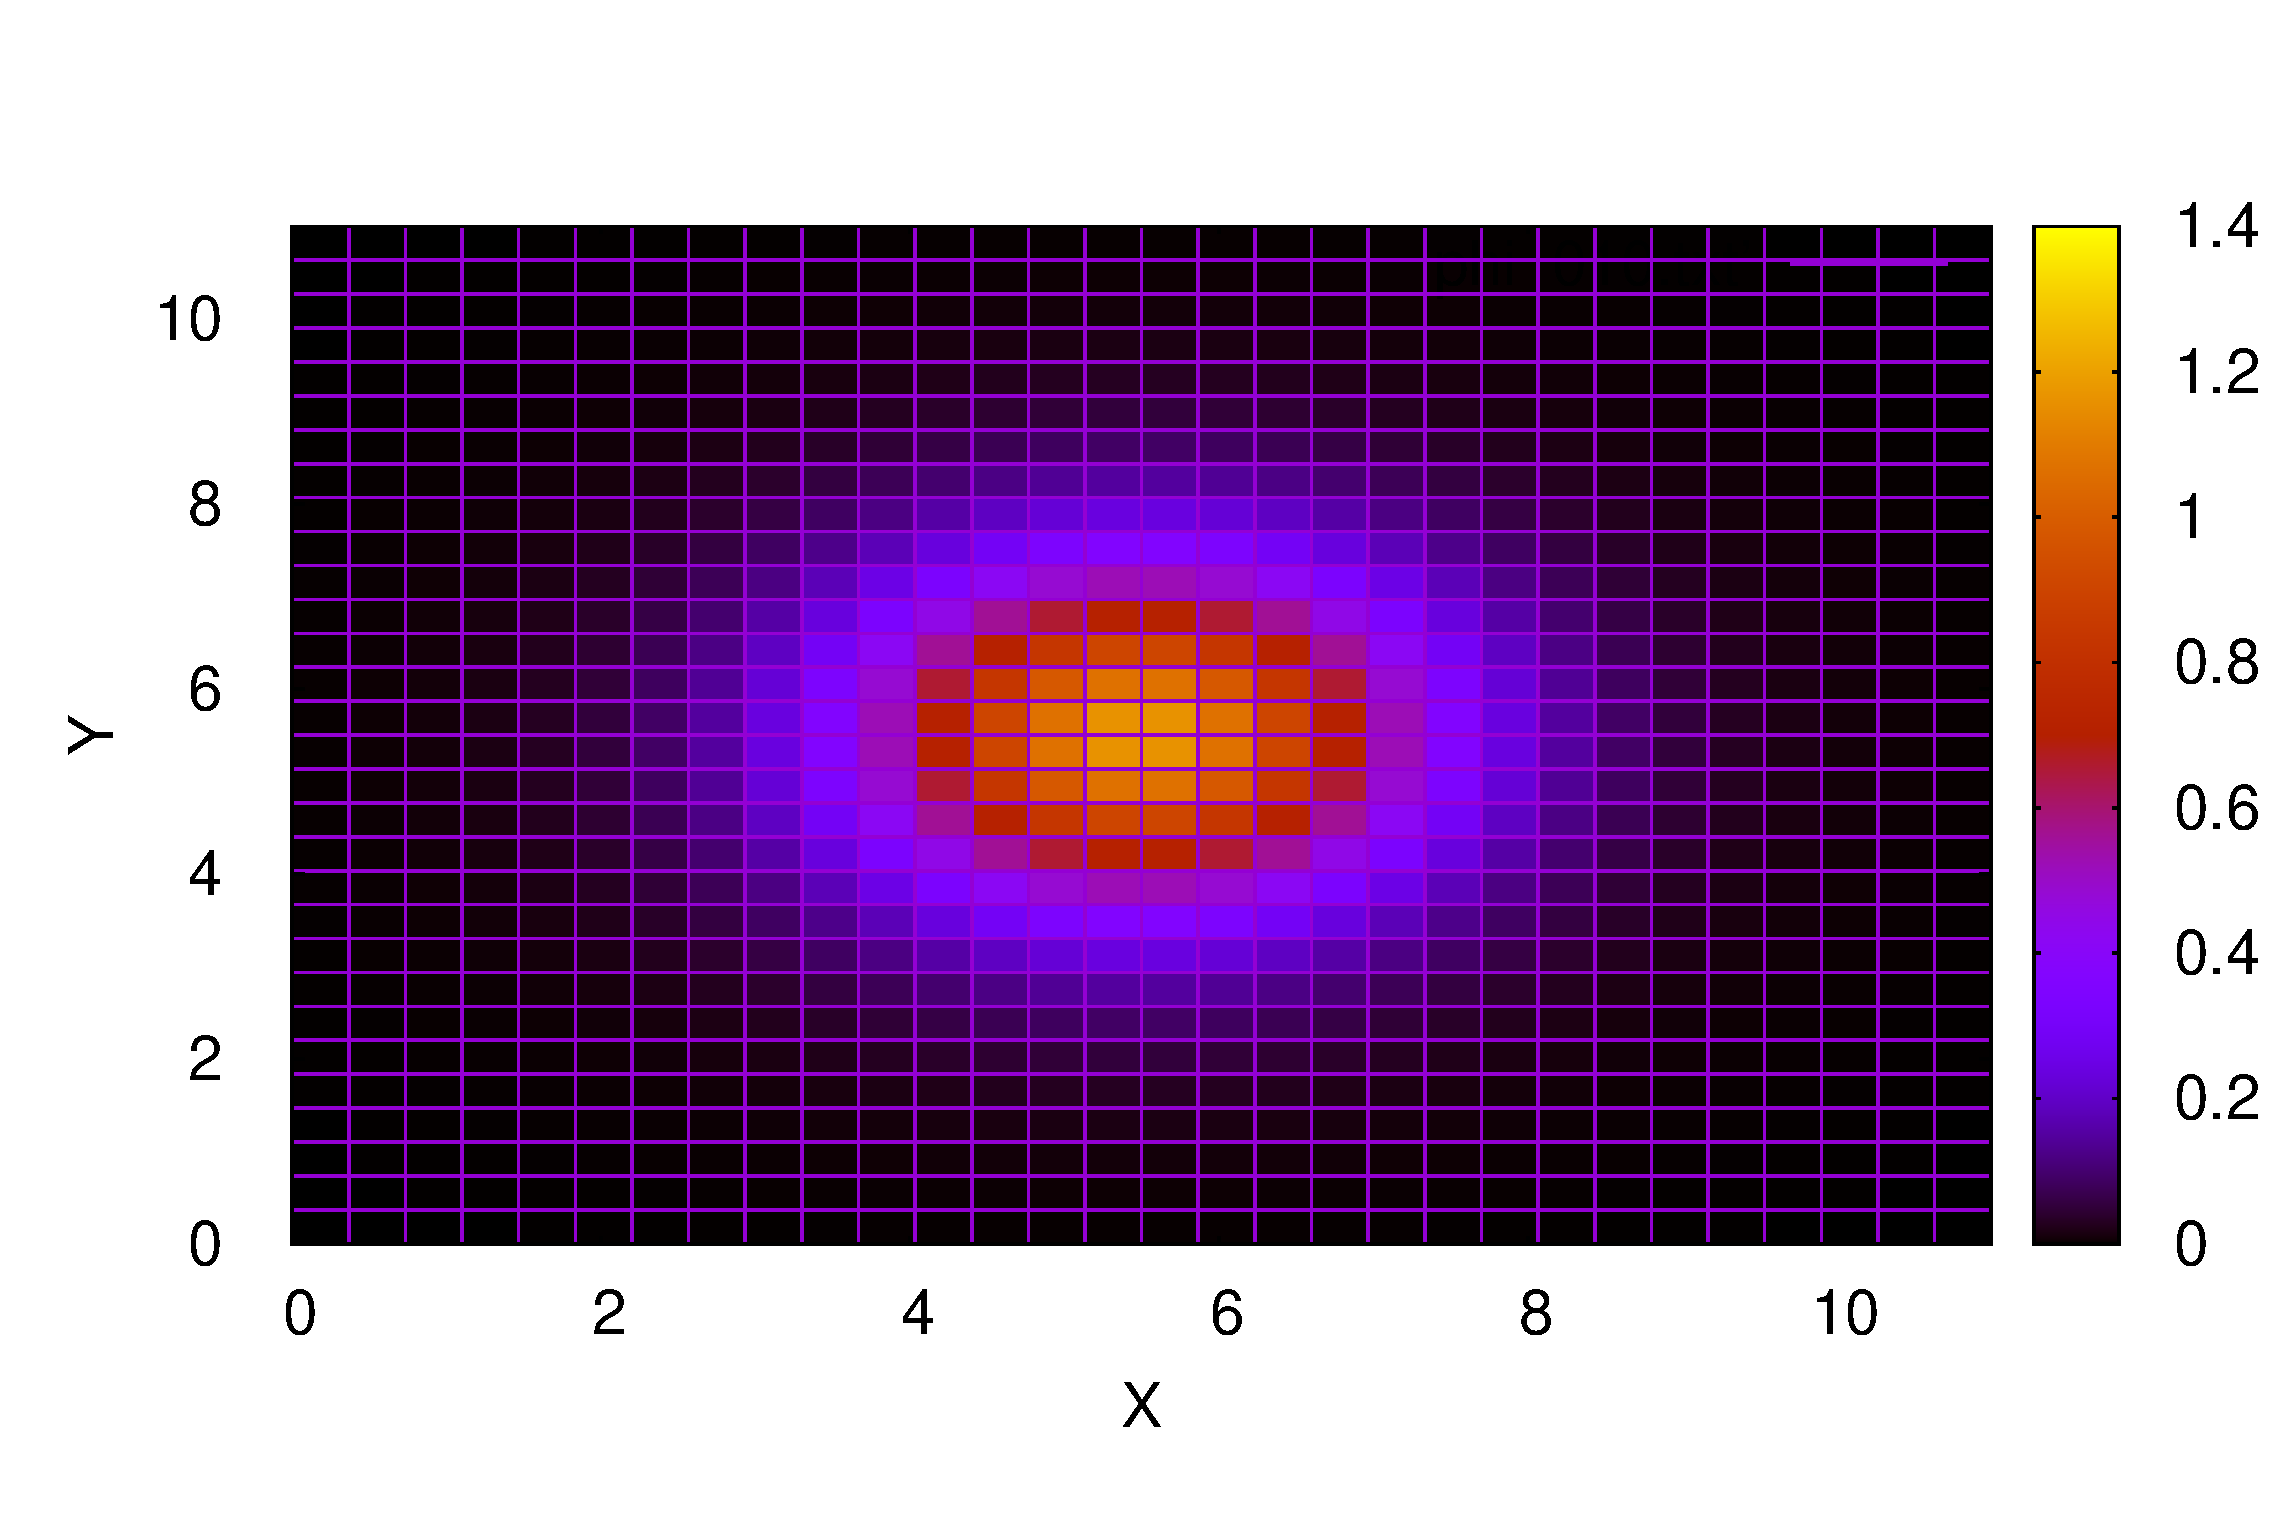
\includegraphics[width=\textwidth]{2DSimplefig/10_map}
		\caption{the heat distribution map after 10 timesteps for the 2D heat problem}
		\label{fig:2d-10dt}
     \end{subfigure}
     \hfill     
        \caption{solving two-dimensional heat equation using CG method.}
        \label{fig:2d-CG}
\end{figure}



In this case (constant diffusion coefficient), it is clear that the diffusion process is symmetric.
 \\

\subsection{The case of random diffusion coefficient}
The initial conditions of this case is the same as the initial condition for the constant diffusion coefficient (figure \ref{fig:2d-initial_condition}). 
\\

\begin{figure}
     \centering
     \begin{subfigure}[b]{0.45\textwidth}
         \centering
         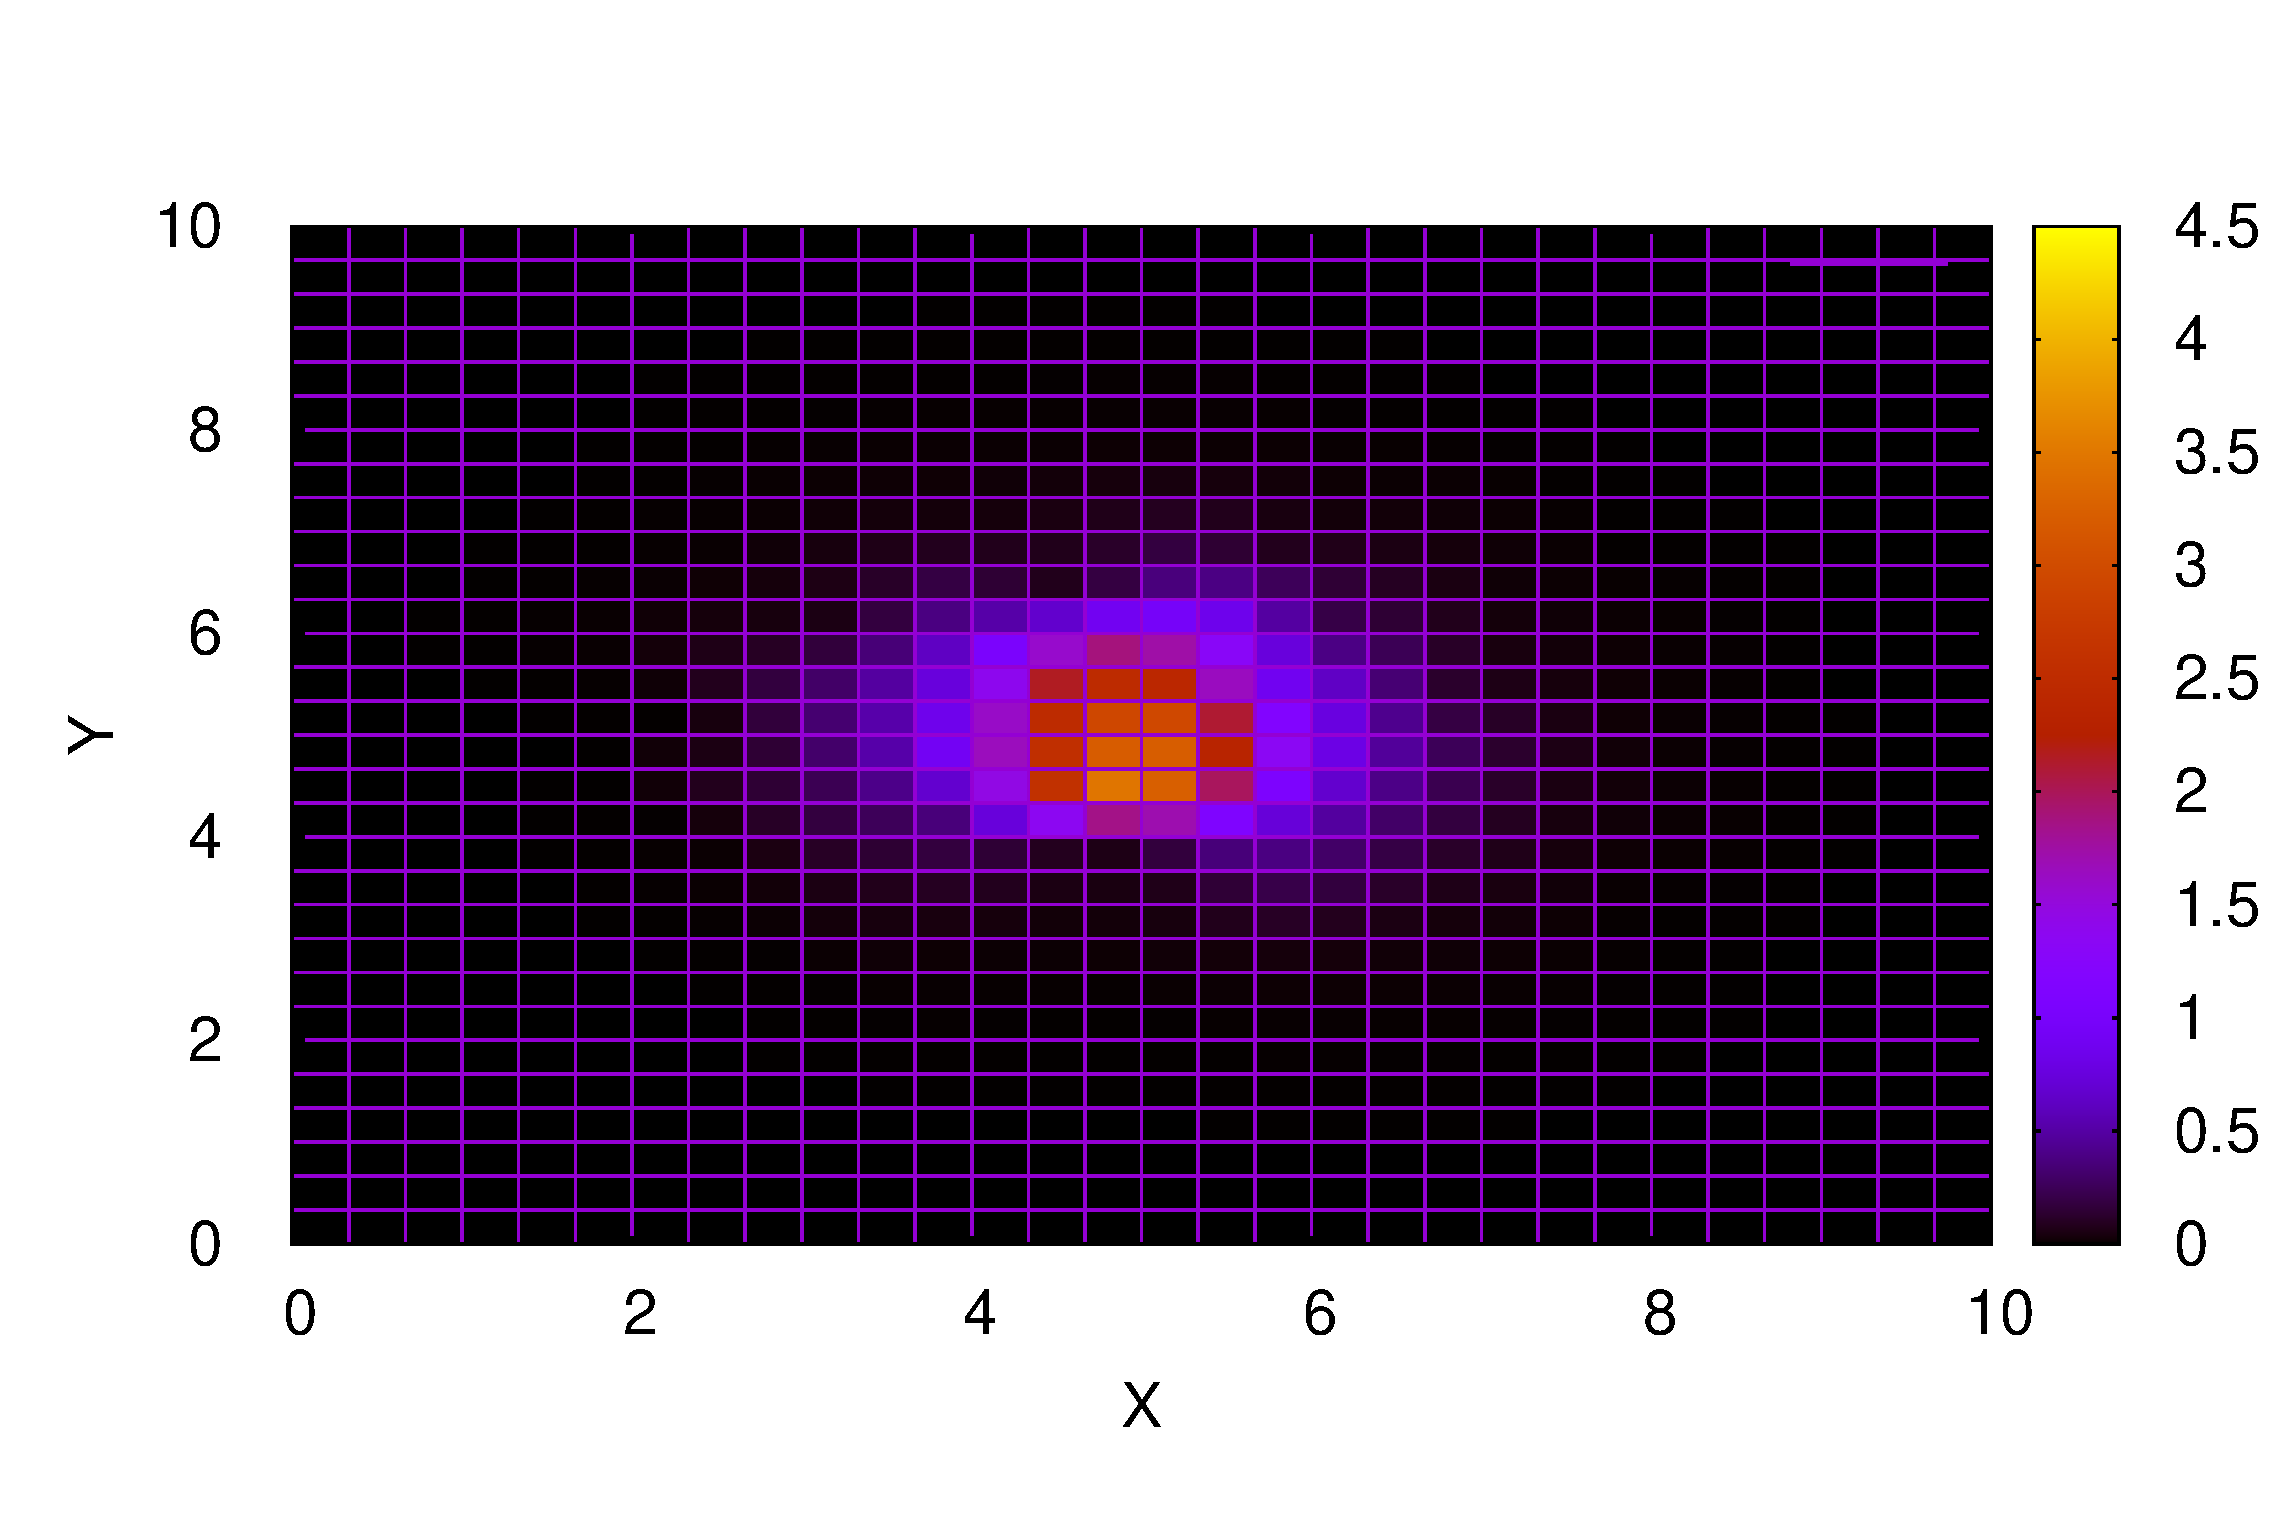
\includegraphics[width=\textwidth]{2DRandomDfig/05_map}
		\caption{the heat distribution map after 5 timesteps for the 2D heat problem}
		\label{fig:2d-randomD-5dt-map}
     \end{subfigure}
     \hfill
	\centering
     \begin{subfigure}[b]{0.45\textwidth}
         \centering
         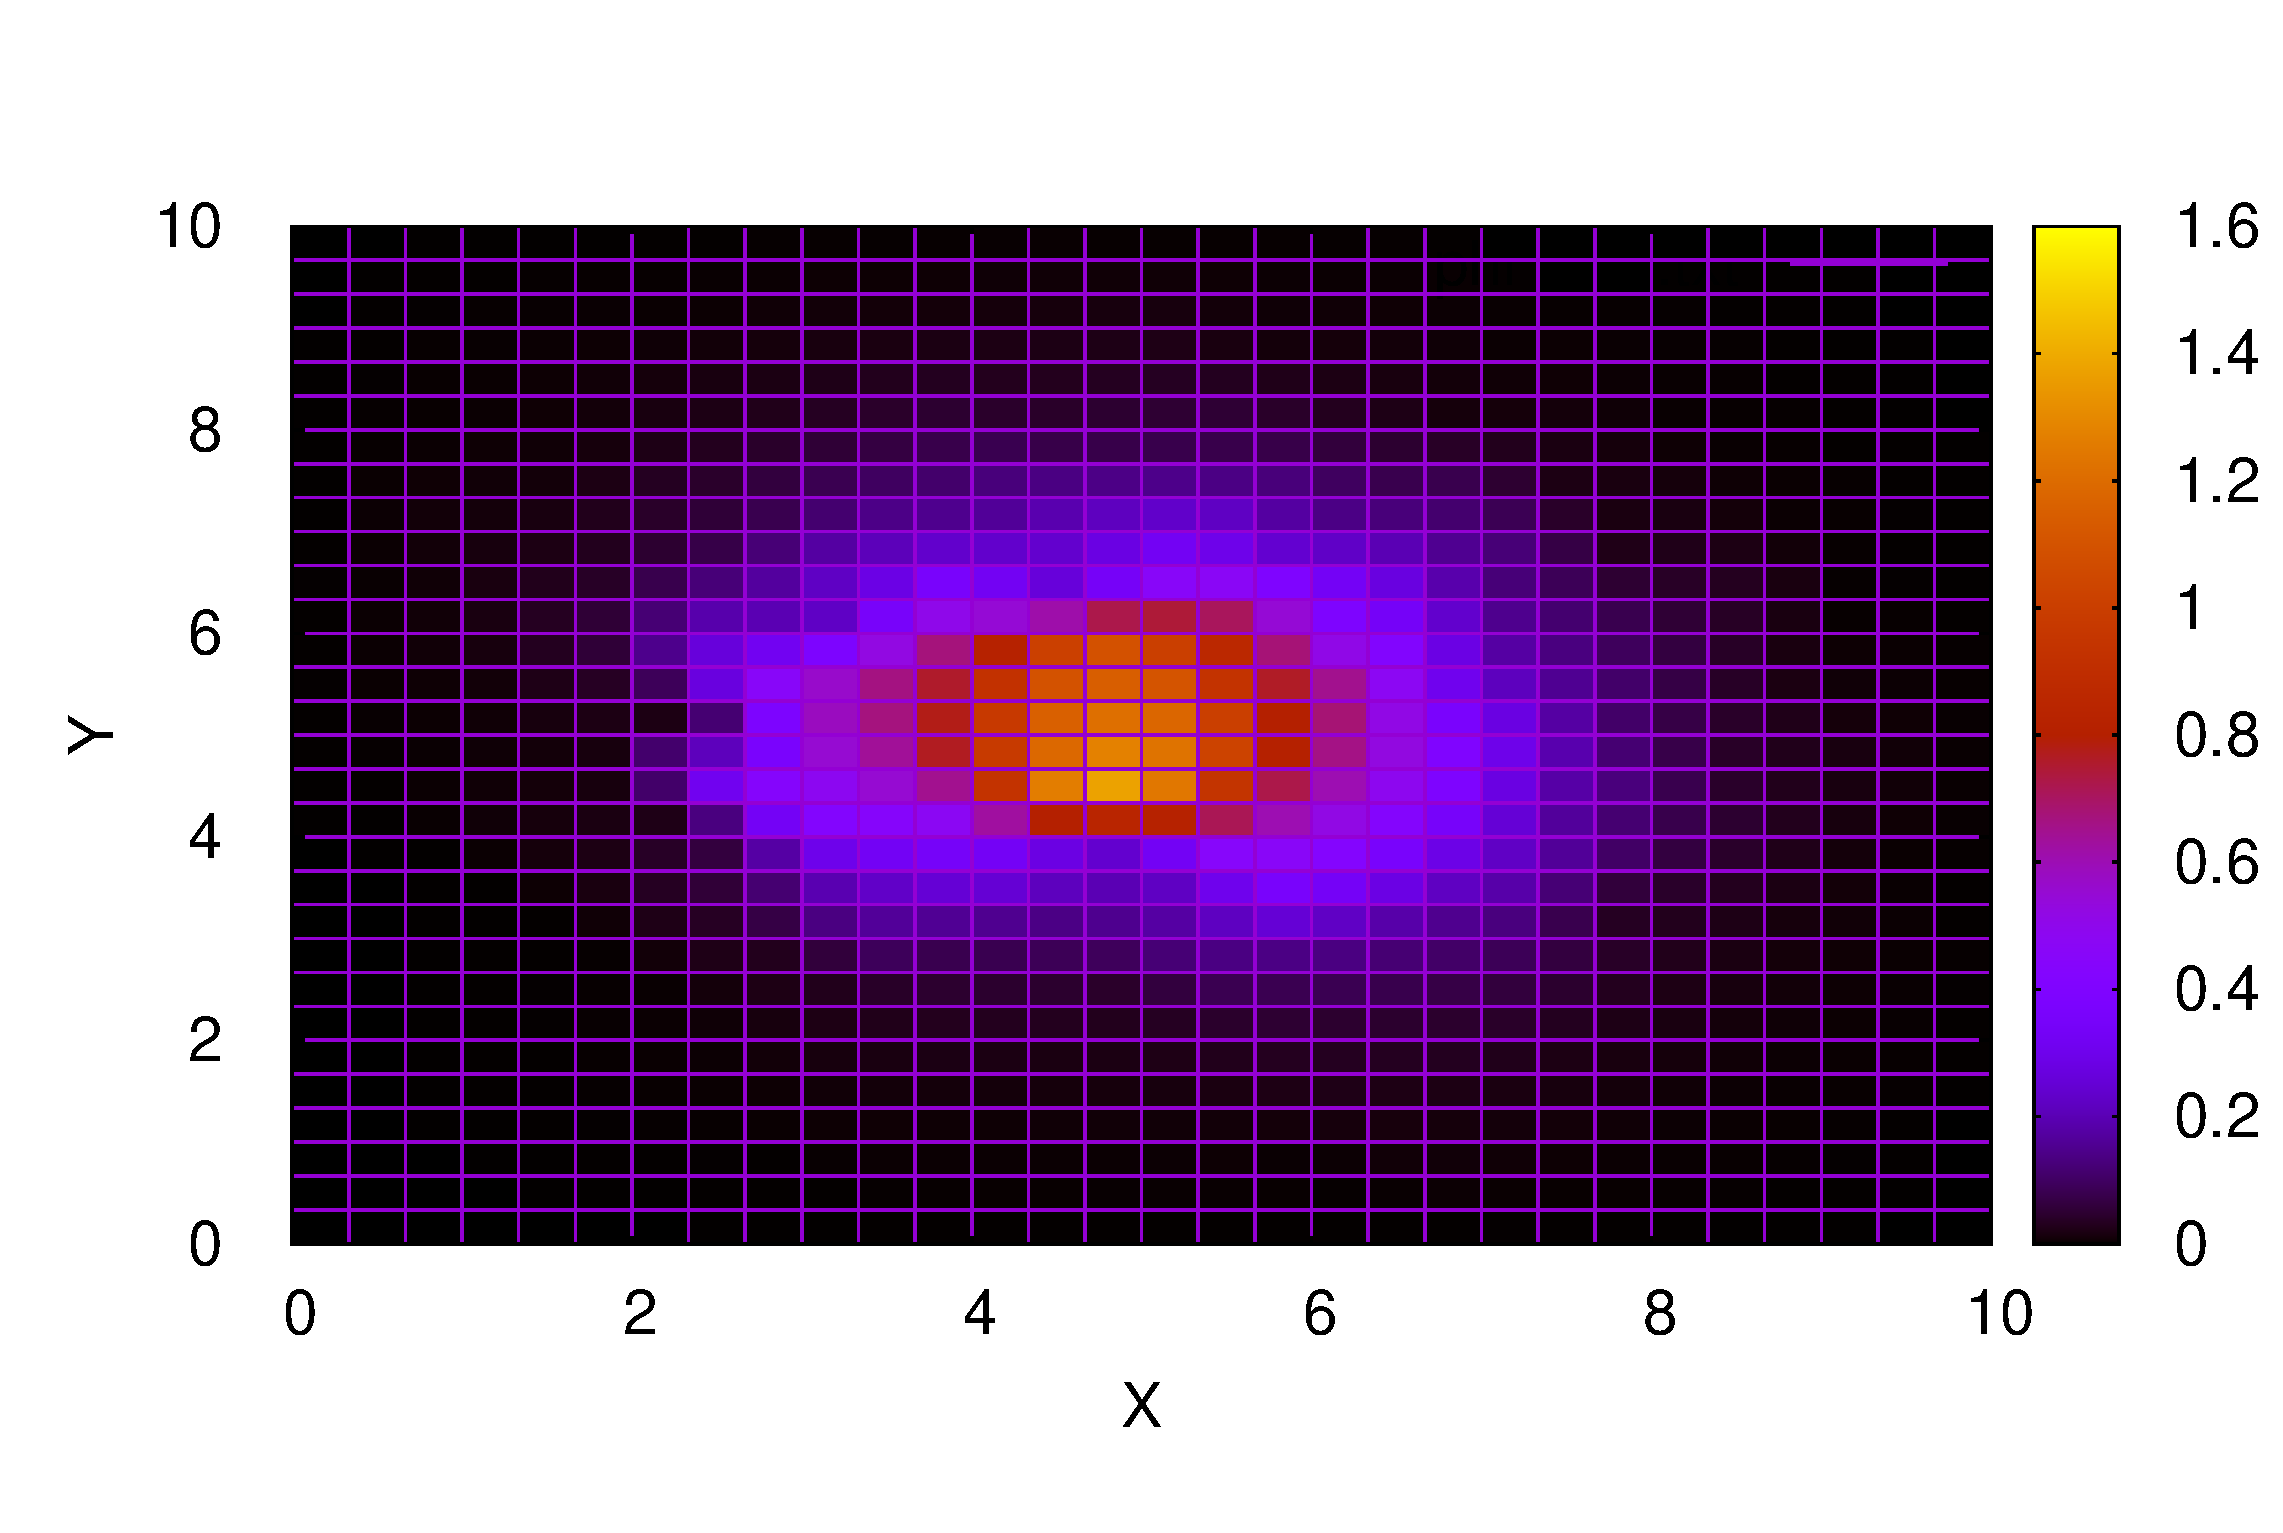
\includegraphics[width=\textwidth]{2DRandomDfig/15_map}
		\caption{the heat distribution map after 15 timesteps for the 2D heat problem}
		\label{fig:2d-randomD-15dt-map}
     \end{subfigure}
     \hfill     
          \begin{subfigure}[b]{0.45\textwidth}
         \centering
         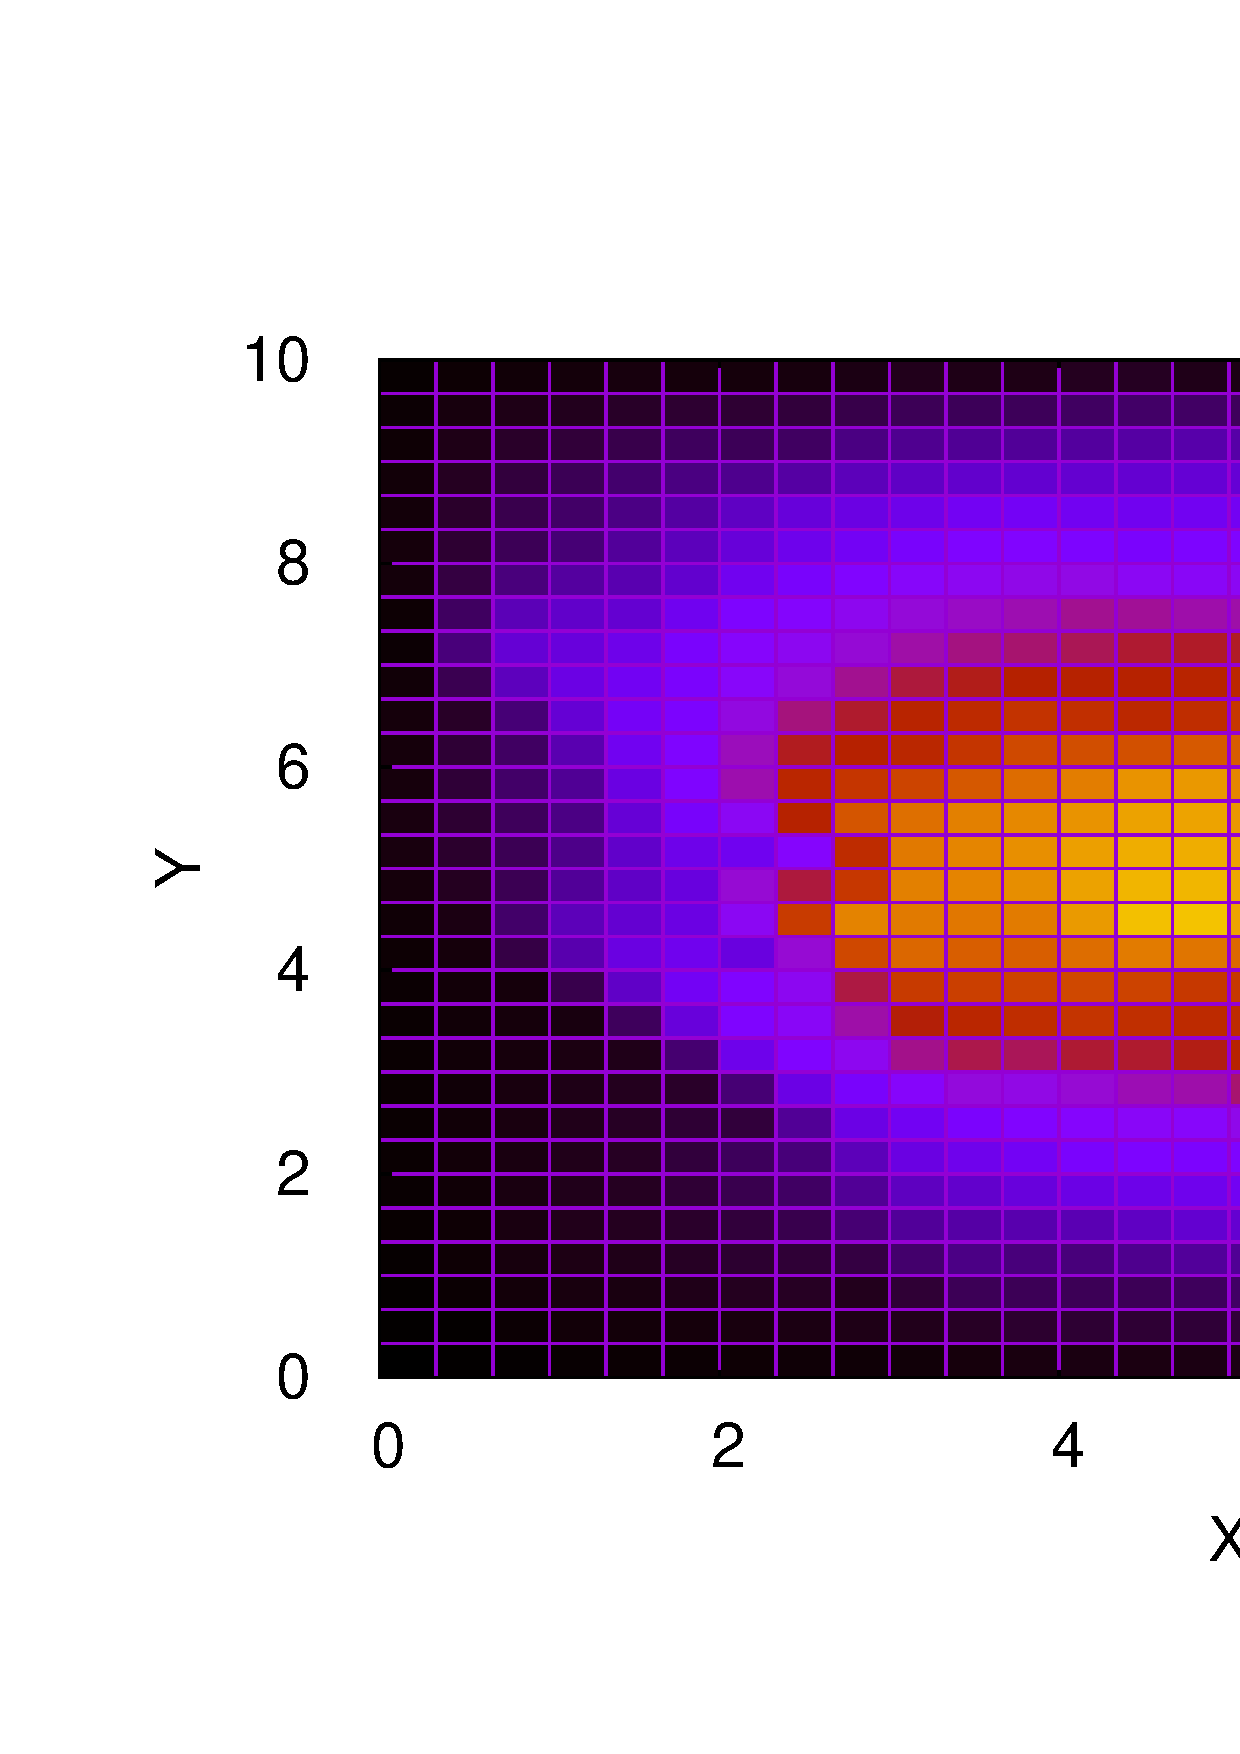
\includegraphics[width=\textwidth]{2DRandomDfig/45_map}
		\caption{the heat distribution map after 45 timesteps for the 2D heat problem}
		\label{fig:2d-randomD-45dt-map}
     \end{subfigure}
     \hfill     
        \caption{solving two-dimensional heat equation using CG method.}
        \label{fig:2d-CG-randomD}
\end{figure}

In contrast with the case of the constant diffusion coefficient, because of those random points which will not diffuse ($D(\vec{r}^{*})=0$), here the distribution of $\phi$ is not symmetric.

%stv
insert the plots for simple 2d and then the assignment here


\phantomsection
\section*{Appendix} % The \section*{} command stops section numbering
\addcontentsline{toc}{section}{Appendix} % Adds this section to the table of contents

As computer architecture advanced, it became more difficult to compare the performance of various computer systems simply by looking at their specifications. Therefore, tests were developed that allowed comparison of different architectures. For example, Pentium 4 processors generally operated at a higher clock frequency than Athlon XP or PowerPC processors, which did not necessarily translate to more computational power; a processor with a slower clock frequency might perform as well as or even better than a processor operating at a higher frequency \footnote{The megahertz myth, or less commonly the gigahertz myth, refers to the misconception of only using clock rate (for example measured in megahertz or gigahertz) to compare the performance of different microprocessors.}.
\\
Benchmarks are designed to mimic a particular type of workload on a component or system. Benchmarking is usually associated with assessing performance characteristics of computer hardware, for example, the floating point operation performance of a CPU.
\subsection*{PARKBENCH}
The PARKBENCH (PARallel Kernels and BENCHmarks) committee, originally called the Parallel Benchmark Working Group (PBWG) was founded at Supercomputing '92 in Minneapolis, when a group of about 50 people interested in computer benchmarking met under the joint initiative of Tony Hey and Jack Dongarra, and the chairmanship of Roger Hockney. The objectives of the PARKBENCH group are; 
\begin{itemize} 
\item To establish a comprehensive set of parallel benchmarks that is generally accepted by both users and vendors of parallel systems.

\item To provide a focus for parallel benchmark activities and avoid unnecessary duplication of effort and proliferation of benchmarks.
\item To set standards for benchmarking methodology and result-reporting together with a control database/repository for both the benchmarks and the results.
\item To make the benchmarks and results freely available in the public domain. 
\end{itemize}
	
Further information on PARKBENCH may be obtained at:\\
 \texttt{http://www.netlib.org/parkbench} .

\subsection*{NAS Parallel Benchmarks}

NAS Parallel Benchmarks (NPB) are a set of benchmarks targeting performance evaluation of highly parallel supercomputers. The NAS Parallel Benchmarks (NPB) are a small set of programs designed to help evaluate the performance of parallel supercomputers.  They are developed and maintained by the NASA Advanced Supercomputing (NAS) Division (formerly the NASA Numerical Aerodynamic Simulation Program) based at the NASA Ames Research Center.
The benchmarks are derived from computational fluid dynamics (CFD) applications and consist of five kernels and three pseudo-applications. The benchmark suite has been extended to include new benchmarks for unstructured adaptive meshes, parallel I/O, multi-zone applications, and computational grids. 
\\
The original eight benchmarks specified in NPB 1 mimic the computation and data movement in CFD applications:
\begin{itemize}
  \item IS - Integer Sort, random memory access
  \item EP - Embarrassingly Parallel
  \item CG - Conjugate Gradient, irregular memory access and communication
  \item MG - Multi-Grid on a sequence of meshes, long- and short-distance communication, memory intensive
  \item FT - discrete 3D fast Fourier Transform, all-to-all communication
  \item BT - Block Tri-diagonal solver
  \item SP - Scalar Penta-diagonal solver
  \item LU - Lower-Upper Gauss-Seidel solver
\end{itemize}
and there are several other benchmarks for unstructured computation, parallel I/O, and data movement.
\\
As of NPB 3.3, eleven benchmarks are defined. Further information on NAS may be obtained at: \\ \texttt{www.nas.nasa.gov/publications/npb.html} .
  
%\input{sections/sample}
%------------------------------------------------

  
\bibliographystyle{unsrt}
\bibliography{ref}

 
\end{document}